\documentclass[11pt,a4paper]{article}
\usepackage[T1]{fontenc}
\usepackage[utf8]{inputenc}
\usepackage{lmodern,microtype,amsmath,amssymb,bm,booktabs,graphicx}
\usepackage[margin=25mm]{geometry}
\usepackage[numbers,sort&compress]{natbib}
\usepackage[colorlinks=true,allcolors=blue]{hyperref}
\hypersetup{pdftitle={MOUSE: Semiempirical Orbital-Optimized DFT with Analytic Gradients and Hessians},pdfauthor={Vincenzo Barone}}
\usepackage{siunitx}
\usepackage{fancyhdr}
\pagestyle{fancy}\fancyhf{}\fancyhead[L]{MOUSE: semiempirical orbital-optimized DFT}\fancyhead[R]{IJQC submission}\fancyfoot[C]{\thepage}
\setlength{\headheight}{14pt}
\renewcommand{\topfraction}{0.90}\renewcommand{\bottomfraction}{0.85}\renewcommand{\textfraction}{0.08}\renewcommand{\floatpagefraction}{0.70}
\newcommand{\npi}{\ensuremath{n\!\rightarrow\!\pi^*}}
\newcommand{\pipi}{\ensuremath{\pi\!\rightarrow\!\pi^*}}
\newcommand{\Eh}{\ensuremath{E_{\mathrm h}}}
\title{Semiempirical Orbital-Optimized DFT in MOUSE:\\Spin-Pure Excited-State Surfaces with Analytic Gradients and Hessians}
\author{Vincenzo Barone\\\small Consorzio Interuniversitario Nazionale per la Scienza e Tecnologia dei Materiali}
\date{5 November 2026}
\begin{document}
\maketitle
\begin{abstract}
Excited-state spectroscopy of large molecules requires a balanced description
of electronic reorganization and nuclear motion. We present a semiempirical
orbital-optimized model in the Molecular Orbital Utility for Semiempirical
Explorations (MOUSE), in which spin-polarized GFN2 (second-generation
geometry, frequency, noncovalent and tight-binding) orbitals are
relaxed on a density functional theory (DFT)-informed energy surface and
singlet excitations are formed
from spin-pure configurations. The excitation energy, forces and vibrational
curvature are obtained from the same state-specific surface. Selected double
excitations and a screened interaction describe the multiconfigurational
character of conjugated chromophores while preserving a compact valence
representation. On 26 states in 24 molecules, the mean absolute error is
0.183 eV with a maximum error of 0.478 eV. The twelve $\pi\!\rightarrow\!\pi^*$
states have a mean absolute error of 0.209 eV, and the fourteen
$n\!\rightarrow\!\pi^*$ states have a mean absolute error of 0.160 eV.
Analytic gradients and Hessians include orbital relaxation, spin recoupling,
configuration-space response, the moving ground-state projector and
state-interaction response. The resulting energy surface supports excited-
state relaxation, vibrational analysis and repeated calculations on extended
chromophores. Carotene and chlorophyllide examples illustrate the treatment of
strongly conjugated pigment manifolds.
\end{abstract}
\noindent\textbf{Keywords:} orbital-optimized DFT; semiempirical quantum
chemistry; excited states; spin-pure ROKS; analytic gradients; analytic
Hessians; DeltaSCF; MOUSE.

\section{Introduction}
The absorption spectrum of a conjugated molecule is determined by the coupled
motion of electrons and nuclei. The transition changes bond orders, charge
distribution and orbital occupations, and the electronic state therefore
relaxes on a geometry different from that of the ground state. Excited-state
structures and vibrational spectra require an energy surface that describes
this relaxation together with its first and second nuclear derivatives. The
same requirement appears in pigment photophysics, where several close-lying
configurations share the visible spectrum and their ordering determines the
observed bands.

A practical description must retain the electronic degrees of freedom of the
chromophore and remain affordable for conformational sampling, solvent
models and multilevel QM/QM$'$ calculations. Semiempirical methods provide
this reach through compact valence Hamiltonians. Their value for excited
states is greatest when the approximation defines a differentiable,
state-specific energy rather than only a vertical transition estimate.
Analytic gradients and Hessians then connect spectroscopy with structures,
relaxation pathways and vibronic observables. Subtractive multilayer
constructions such as ONIOM provide an established framework for combining
quantum levels.\cite{oniom2015}

The field includes simplified response theories such as sTDA, sTDA-xTB and
the recent std2 family, DFTB-based response and $\Delta$DFTB, TDDFT+TB,
TDDFT-aas, and semiempirical multireference methods based on OMx/ODMx.
\cite{tda,stdft2014,stdaxtb2016,std22026,dftb2025,deltadftb2016,tbgrad2023,aas2024,omxexc2016,odmx2019}
These methods establish complementary routes to efficient spectra, excited-
state gradients and multiconfigurational wave functions. The present work
focuses on the state-specific energy surface generated by orbital relaxation
and its analytic nuclear response.

Simplified Tamm--Dancoff and TD-DFT methods describe many transitions from a
ground-state reference and are effective for broad spectral surveys.\cite{tda,stdft2014,stdaxtb2016}
State-specific orbital optimization provides a complementary description: a
non-Aufbau occupation defines the excited configuration, the orbitals relax in
its field, and the transition energy is the difference between stationary
ground- and excited-state energies. In $\Delta$SCF and orbital-optimized DFT,
this relaxation is central to charge-transfer, $n\!\rightarrow\!\pi^*$ and
strongly reorganized $\pi\!\rightarrow\!\pi^*$ states.\cite{mom2008,hait2021}
The excited solution is an electronic stationary point and often a saddle;
direct orbital optimization and saddle searches therefore provide a natural
route to state following.\cite{levifaraday,levi2020,ivanov2021,gmf2023}

State-specific optimization is already possible at the semiempirical level. In particular, $\Delta$DFTB provides self-consistently optimized excited-state energies and gradients, with applications to structures, Stokes shifts and vibrational frequencies.\cite{deltadftb2016} The opportunity addressed here is therefore more specific than introducing semiempirical $\Delta$SCF. We seek a DFT-informed semiempirical OO-DFT surface with explicit spin polarization, a spin-pure singlet representation, and complete analytic response through the nuclear Hessian. For a single targeted state, such a formulation allows the existing ground-state engine to supply most of the electronic machinery, while the excited-state solver supplies occupation control, orbital stationarity and its constrained response. For interacting or strongly mixed configurations, an additional state-interaction treatment is required.

Our organizing principle is to separate the standard ground-state DFT calculation from the less expensive calculation of the excitation response or energy increment. Writing $\Delta E_I=E_I-E_0$ distinguishes the description of the absolute ground-state energy from the description of the change produced by excitation. In a multilevel application, this separation can be expressed schematically as $E_I^{\rm composite}=E_0^{\rm DFT}+\Delta E_I^{\rm low}$: standard DFT supplies the baseline, while a compact quantum model supplies the state-dependent increment. This expression is a design principle for combining levels of theory, rather than an assumption that the two terms have the same approximation error. It also requires consistent differentiation of both contributions when forces or frequencies of the composite surface are needed.

In the present MOUSE formulation, a conventional DFT program prepares ground-state orbital-reference information and response operators at an anchor geometry. These quantities are transferred to a native GFN2-based valence representation and then used by a separate prepared excited-state calculation.\cite{gfn2} The native spatial orbitals remain the variational variables. Ground and excited states are made stationary in a common prepared semiempirical energy, and their difference defines the reported excitation increment. This provides a concrete separation between external reference preparation and runtime evaluation: the latter uses the semiempirical engine and stored operators, without a new DFT or TDA calculation. Reuse of the prepared operators away from the anchor is an approximation whose range must be validated. The multilevel motivation likewise does not imply that an additional DFT ground-state calculation is included in every benchmark timing.

MOUSE implements this strategy with a spin-polarized native energy and a
restricted-open-shell Kohn--Sham (ROKS) singlet construction.\cite{roks1998}
A coherent combination of exchanged-spin determinants defines a spin-pure
configuration state function (CSF); its orbitals satisfy the constrained
excited-state stationarity equations. Selected singlet double excitations are
coupled through a prepared screened interaction to describe configuration
mixing beyond a single optimized promotion. The resulting surface requires
the response of the stationary orbitals, constraint multipliers, nonorthogonal
configuration metric, ground-state projector and state-interaction
eigenvector. These contributions give analytic gradients and Hessians of the
energy used for the spectrum.

This work establishes the semiempirical OO-DFT formulation and its analytic
implementation in MOUSE. TDA is evaluated on the same corrected native GFN2
orbitals and reference preparation, allowing the role of orbital relaxation
and state interaction to be measured directly. The study covers vertical
excitation energies, state following, analytic derivatives and conjugated
pigment manifolds. Figure~\ref{fig:workflow} summarizes the relation between
the molecular excitation, the state-specific energy surface and its nuclear
response.

\begin{figure}[!htbp]
\centering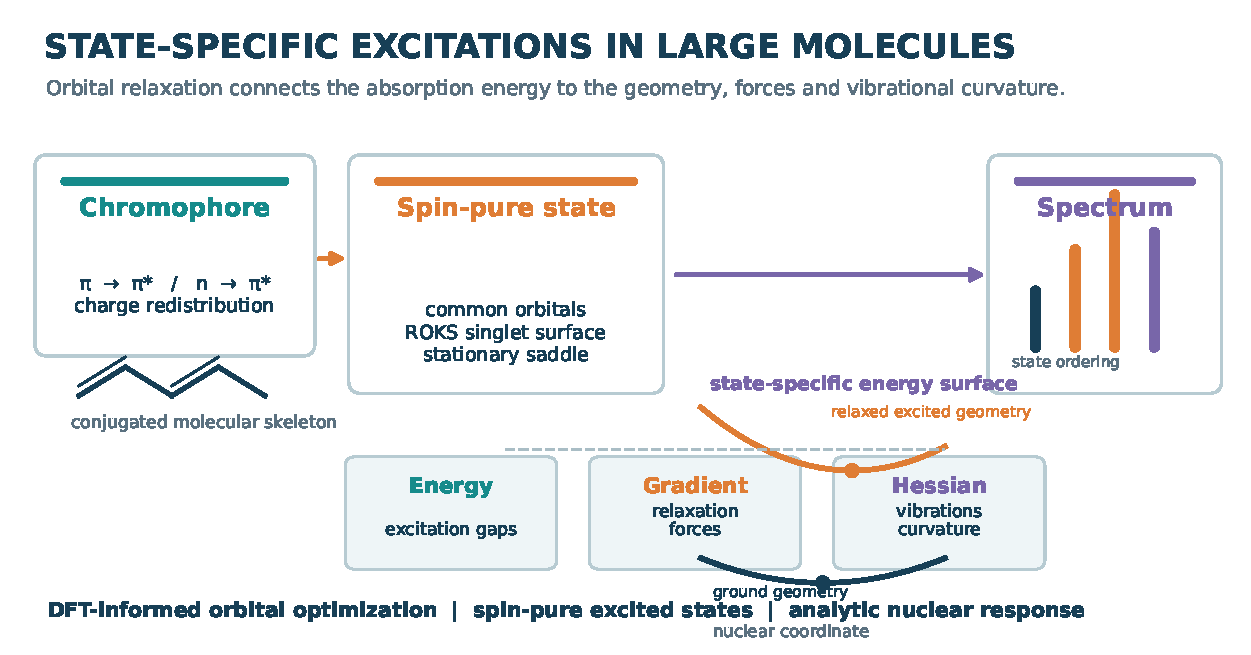
\includegraphics[width=\linewidth]{figures/graphical_abstract_ijqc.pdf}
\caption{Chemical and spectroscopic picture of the MOUSE excited-state surface. Orbital relaxation converts a vertical excitation into a state-specific energy surface that supplies the absorption energy, relaxed forces and vibrational curvature. Spin-pure singlet configurations and their interaction describe the ordering and intensity pattern of conjugated chromophores.}\label{fig:workflow}
\end{figure}

\section{Theory and implementation}
\subsection{Common reference and spin-polarized native energy}
The native GFN2 spatial orbitals $C_{\rm n}$ define the retained valence
orbital space. At the frozen anchor, a core-orthogonal isometry embeds this
space in the
DFT AO space. The diagonal Rayleigh quotients of the embedded DFT Fock matrix
supply levels $F_i$. Qualified occupied/virtual assignments transfer DFT
orbital spacings to $Q_i$ after aligning occupied centroids; levels without a
levels retain $F_i$. The correspondence thresholds are 0.7 in absolute
overlap and 0.05 in best-versus-alternative margin. If the molecular Q
transfer loses its occupied--virtual gap, Q reverts to F. The common
one-body reference uses $\epsilon_i=(F_i+Q_i)/2$ before orbital optimization.
DFT spatial orbitals are not substituted for the native orbitals. This is
not an arithmetic average of two independently optimized excited energies.

In a complete symmetric AO-pair moment representation, the prepared energy is
\begin{align}
 E[P^\alpha,P^\beta;R]&=E_{\rm native}
 +v^{\mathsf T}q+\tfrac12(q-q_0)^{\mathsf T}K_c(q-q_0)
 +\tfrac12m^{\mathsf T}K_s m,\\
 q_a&=\operatorname{Tr}[B_a(P^\alpha+P^\beta)],\qquad
 m_a=\operatorname{Tr}[B_a(P^\alpha-P^\beta)].
\end{align}
$E_{\rm native}$ retains the native electronic, charge-dependent,
anisotropic, repulsive, dispersion and spin-polarization terms; $K_c$ and
$K_s$ are the prepared additional response corrections. The charge correction
subtracts the corresponding native response rather than adding a duplicate
Coulomb kernel. The linear term places the reference Fock spectrum in the
native orbital space. The quadratic tensors are prepared at the stationary embedded
DFT density and the linear reference is centered on the native ground.
Spin polarization is part of the energy and its derivatives, not an additive
excitation correction.

The final reference is CAM-B3LYP,\cite{camb3lyp2004} with range parameter
$0.33\,{\rm bohr}^{-1}$. The inherited uracil scale $\lambda=0.9$ multiplies
its exact-exchange response once, giving short- and long-range response
coefficients 0.171 and 0.585. The semilocal response is unchanged and orbital
gaps are not multiplied by $\lambda$. Neither operator construction nor
state assignment uses a reference excitation energy.

\subsection{Spin purity and electronic saddle stationarity}
For a promotion $h\to p$, the two exchanged-spin determinants sharing a
single spatial orbital set define a singlet CSF with a consistent fermion
phase convention. Its energy is the restricted-open-shell multiplet sum
\begin{equation}
 E_S(C,R)=2E_M(C,R)-E_T(C,R).
\end{equation}
The singlet CSF is spin pure, whereas the density-functional multiplet-sum
energy remains approximate. This does not identify a broken-symmetry
$M_s=0$ determinant as an exact singlet. Four-open-shell occupations require
two independent singlet recouplings, both retained below.

The ground is made stationary in the native closed-shell functional. Target
ROKS orbitals satisfy the ground-CSF orthogonality constraint and their
bordered stationarity equations. Metric-preserving orbital rotations,
Newton residual searches, and state-overlap guards locate the assigned
branch. An excited solution may be an electronic saddle, as emphasized in
the direct-optimization work of Levi and co-workers;\cite{levi2020,gmf2023}
no orbital-energy minimum is assumed. Electronic saddle order and nuclear
vibrational stability are distinct properties.

Figure~\ref{fig:saddle} illustrates the distinction between electronic
stationarity and nuclear relaxation.

\begin{figure}[tbp]\centering
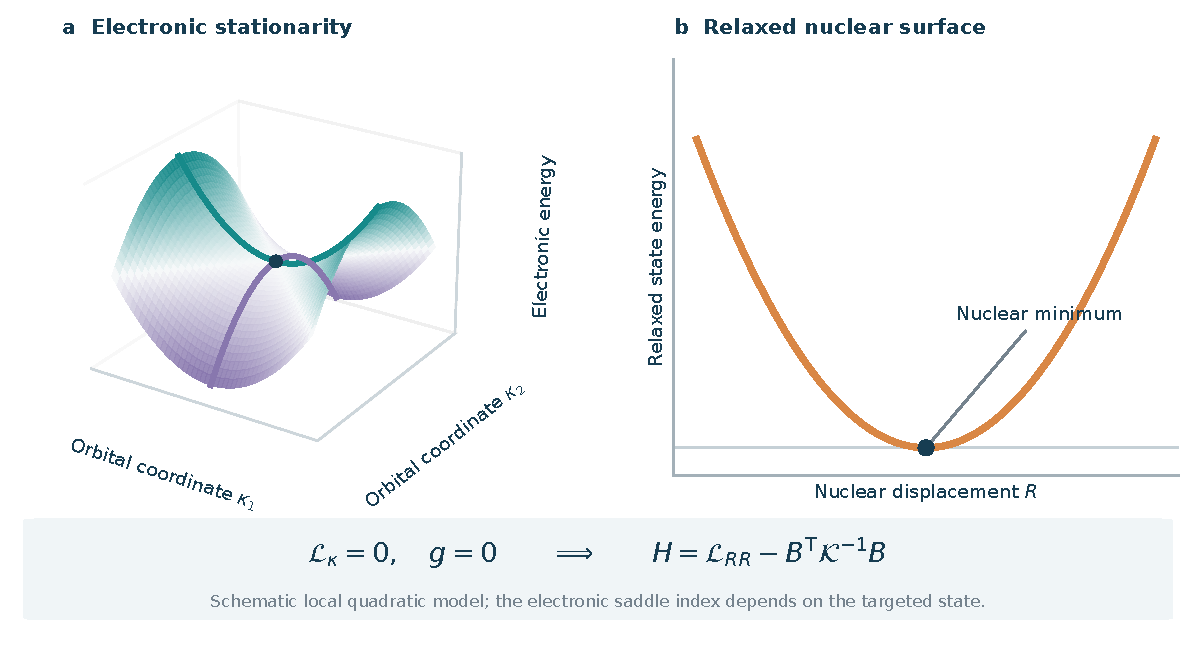
\includegraphics[width=\linewidth]{figures/stationary_response.pdf}
\caption{Electronic saddle character and relaxed nuclear curvature are
distinct properties of an excited-state surface.}\label{fig:saddle}
\end{figure}

\subsection{Analytic response of the state-interaction surface}
Let $z$ collect the stationary ground and target orbital coordinates and
constraint multipliers, and write their residual equations as
$F(z(R),R)=0$. Their first and second analytic responses obey
\begin{align}
 F_z z_a&=-F_a,\\
 F_z z_{ab}&=-F_{ab}-F_{az}z_b-F_{bz}z_a-F_{zz}[z_a,z_b].
\end{align}
The bordered linear systems are solved on the regular assigned branch.
Both responses are required: the subsequent state-interaction eigenvalue
is not stationary with respect to the individually optimized ROKS orbitals.
A variational single-determinant Hessian formula alone would omit terms.

For the generalized eigenproblem in the moving ground-orthogonal space,
$Hc=\mathcal E Sc$ with $c^{\mathsf T}Sc=1$, total matrix derivatives give
\begin{align}
 \mathcal E_a&=c^{\mathsf T}(H_a-\mathcal E S_a)c,\\
 \mathcal E_{ab}&=c^{\mathsf T}(H_{ab}-\mathcal E S_{ab})c
 -\mathcal E_b c^{\mathsf T}S_a c-\mathcal E_a c^{\mathsf T}S_b c\nonumber\\
 &\quad+2\sum_{k\ne n}
 \frac{[c_k^{\mathsf T}(H_a-\mathcal E S_a)c]
 [c_k^{\mathsf T}(H_b-\mathcal E S_b)c]}{\mathcal E-\mathcal E_k}.
\end{align}
Here the derivatives include the orbital/multiplier responses, metric,
transported operators, and moving ground projector. The relevant metric
and eigenvalue separations must be resolved. The absolute excited-state
energy defines molecular forces and curvature; vertical excitation energies
subtract the stationary native ground. Finite differences enter only the
independent validation of these analytic derivatives.

\section{Computational protocol}
The assessment contains 26 valence transitions in 24 molecules. Reference
energies are the QUEST theoretical best estimates.\cite{quest,quest2025}
Molecular geometries and target identities are fixed throughout the
assessment, which spans carbonyl, heteroaromatic and conjugated chromophores.

The prepared CAM-B3LYP references retain the archived aug-cc-pVDZ AO basis,
numerical grid level 3, frozen core embedding, and native valence space.
DFT transition information supplies assigned-state seeds and character checks.
Completed references, stationary states and operators are reused.

The calculations were performed on verified remote compute hosts. Runtime
property checks use two BLAS threads per process. The parallel nuclear-column
validation limits concurrent processes and preserves every completed column.

Matched TDA controls use the same stationary native GFN2 spatial orbitals,
F/Q one-body preparation, density-response kernel and $\lambda=0.9$:
\begin{equation}
 A_{ia,jb}=(\epsilon_a-\epsilon_i)\delta_{ij}\delta_{ab}+K_{ia,jb}.
\end{equation}
The complete nonlocal singlet $A$ operator is used, including the exchange
contribution missing from a real symmetrized static response. These controls
are distinct from published sTDA-xTB and from a separately optimized TDA
parameterization. The screened interaction introduced below is an additional
ingredient of OO-CID, not a hidden modification of the reported TDA values.

\section{Screened, symmetry-augmented optimized-target CID}
The final development candidate addresses the two remaining $\pi\pi^*$
outliers by changing the configuration space and its interaction, while
retaining the native GFN2 orbitals, the same prepared F/Q one-body reference,
50/50 weights, $\lambda=0.9$, and zero excitation-energy offset. It combines
optimized ground-orthogonal ROKS target singlets, their paired doubles,
and the original two-occupied/two-virtual frontier doubles in both reflection
parities. The added configurations are all spin-singlet doubles from the
five highest occupied and five lowest virtual canonical native orbitals
that are even under reflection in the molecular plane. Both independent
singlet recouplings of every four-open-shell occupation are included.
Canonical paired doubles with retained-CSF overlap at least 0.7 are
omitted by the unchanged duplicate-removal rule.
An exact Gaussian-overlap representation certifies the nuclear reflection
and canonical MO parities at preparation. The resulting configuration list
is frozen during subsequent nuclear displacement; it is not reclassified
when an out-of-plane coordinate changes. If reflection or MO parity cannot
be certified, no additional symmetry-sector configuration is selected.

This is one common CSF space and one effective matrix for all requested
states of a molecule. No $n\pi^*$/$\pi\pi^*$ label, reference excitation
energy, molecular exception, or fitted damping factor enters the selection.
For the planar examples, $\pi\pi^*$ targets are reflection-even, whereas
$n\pi^*$ targets are reflection-odd. The symmetry augmentation therefore
adds the missing even-sector flexibility without introducing the large
odd-sector manifold that overcorrelated several controls in the unrestricted
five-pair diagnostic. The choice was made after inspecting the exposed
twenty-state development set and was frozen in commit \texttt{2d59ab8}.
It is a model-development choice, not blind validation or a general prescription
for nonplanar molecules, CT, or Rydberg excitations.

\begin{figure}[p]\centering
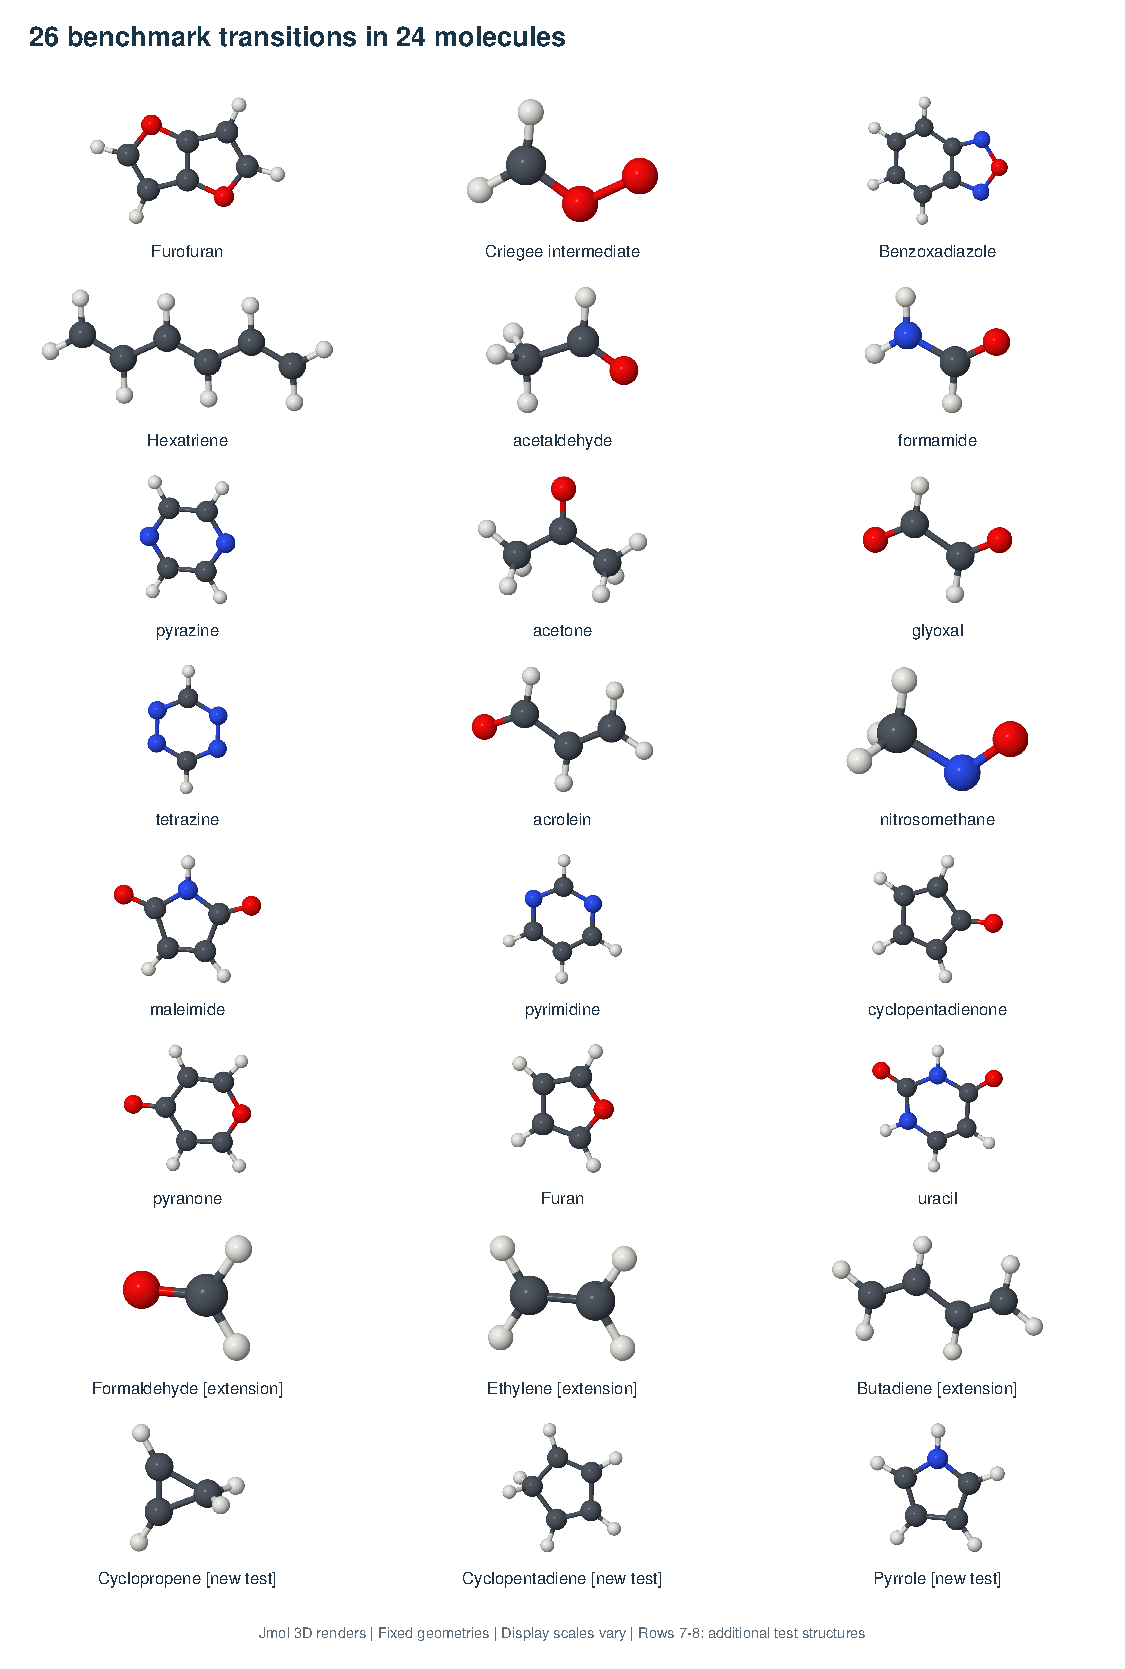
\includegraphics[width=.98\linewidth,height=.83\textheight,keepaspectratio]{figures/screened_cid_structures_jmol.pdf}
\caption{The twenty-four molecular anchors used for the twenty-state development
set and its two three-state extensions, rendered with Jmol from the archived three-dimensional coordinates.
Only rigid display rotations are applied; panel scales differ. Furofuran
contributes two $\pi\pi^*$ states, and Criegee contributes one state of each
valence class.}\label{fig:screenedstructures}
\end{figure}

Environmental screening is introduced through a static finite-basis partition
motivated by constrained RPA.\cite{crpa2004} Let $V$ be the bare Coulomb
matrix in the orthonormal AO-pair chart, $\Delta$ the positive native
occupied--virtual gap matrix, and $T$ the symmetrized transition-density
columns weighted by their environmental fraction. With occupied and virtual
active projectors $P_h,P_v$, these fractions are
$1-(P_h)_{ii}(P_v)_{aa}$; the projectors span the five-pair frontier and
retained optimized hole/particle directions. Our prepared static interaction is
\begin{equation}
 W=V-VT(\Delta+T^{\mathsf T}VT)^{-1}T^{\mathsf T}V.
\end{equation}
This explicitly specified finite-basis approximation is not a full
frequency-dependent cRPA calculation. The same $W$ acts in both reflection
sectors. Its one-body term is normal ordered to the unchanged native reference
Fock matrix, $h_W=F_{\rm ref}-J_W[P_g]+K_W[P_g]/2$.
Let $H^W_{IJ}$ and $S_{IJ}$ denote its Slater--Condon matrix and CSF metric.
The native spin-polarized functional supplies each diagonal energy $E_I$,
and the effective matrix is
\begin{equation}
 H_{IJ}=H^W_{IJ}+\tfrac12S_{IJ}(d_I+d_J),\qquad
 d_I=E_I-H^W_{II}/S_{II}.
\end{equation}
Every two-dimensional four-spin singlet block is restored to the exact
SU(2) completion of the same quadratic spin functional. Excited CSFs are
projected orthogonal to the moving stationary ground CSF before solving
the generalized eigenproblem. Excitation energies subtract its native
stationary energy, not an auxiliary correlated-ground eigenvalue.
The overlap-weighted residual remains an approximate multistate functional;
it is not a proof of a universally balanced correlated ground-state theory.

All seven $\pi\pi^*$ targets now satisfy the unchanged 0.5 eV individual
criterion: their MAE is 0.180 eV and maximum absolute error is 0.349 eV.
Furan changes from 5.804 to 6.609 eV against 6.530 eV, and uracil from
6.080 to 5.259 eV against 5.381 eV. The thirteen $n\pi^*$ controls remain
within 0.5 eV, with 0.250 eV MAE and 0.498 eV maximum error. Overall,
the twenty states give 0.225 eV MAE. These are exposed-data development
results: the earlier post-freeze designation does not make them prospective
tests of this newly selected model. The matched native-orbital TDA control
retains its 0.925 eV MAE, using the same F/Q preparation and native response
kernel; the new screened interaction is an additional ingredient of OO-CID.
This comparison does not establish superiority to every calibrated TDA,
sTDA-xTB, or TD-DFTB parameterization. All individual values are in the
Supporting Information.

\begin{figure}[tbp]\centering
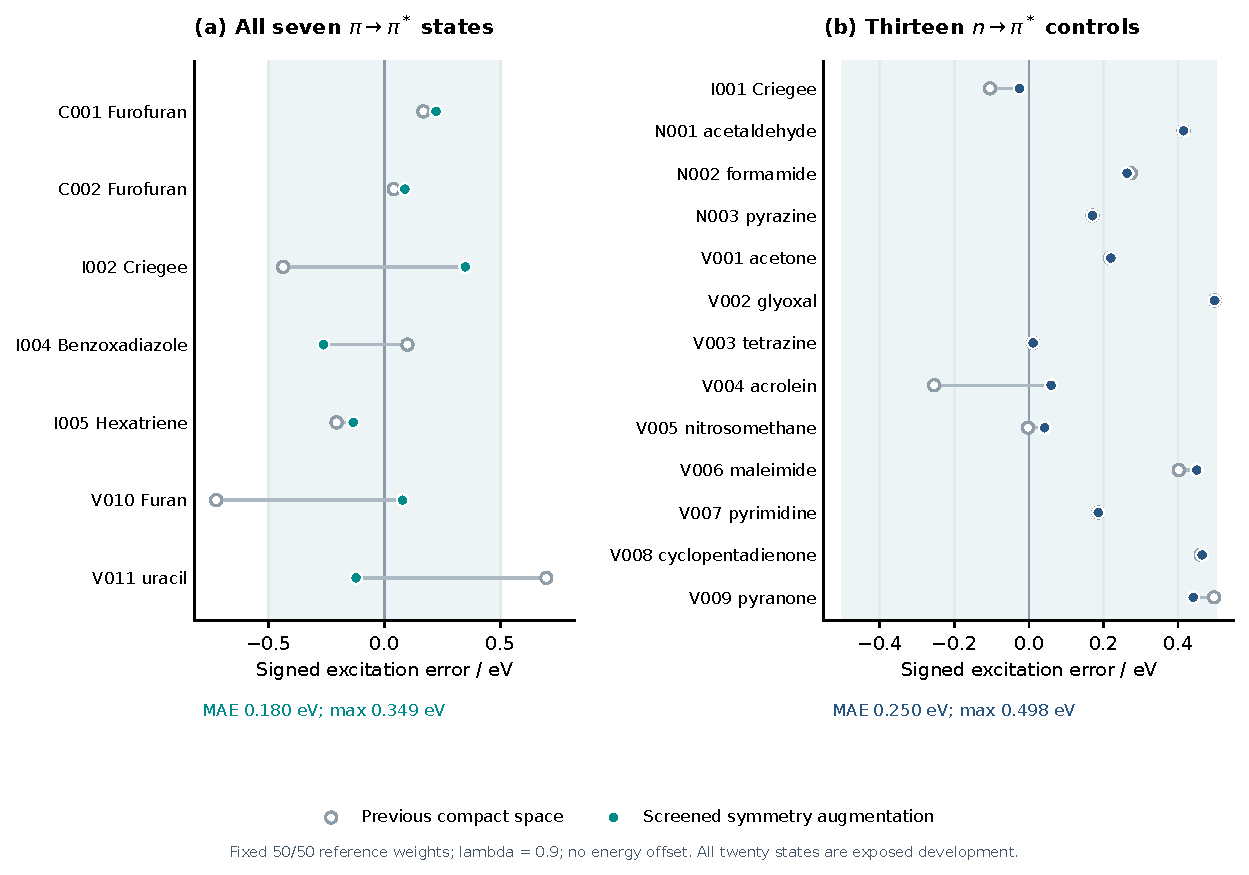
\includegraphics[width=\linewidth]{figures/screened_cid_validation.pdf}
\caption{Resolution of the seven $\pi\pi^*$ development targets while
retaining the thirteen $n\pi^*$ controls. Open circles show the previous
compact-space errors; filled circles show the screened symmetry augmentation.
The shaded interval is $\pm0.5$ eV. All twenty states informed the development
assessment; this figure is not a blind-validation result.}\label{fig:screenedaccuracy}
\end{figure}

The public \texttt{PreparedNOSIModel} accepts a checksummed extended model,
and LINK retains its \texttt{nosi\_50\_50} selector and accepted-restart
contract. Runtime evaluation reuses only ground-engine Fock, energy,
spin-polarization, and derivative primitives; it performs no TDA solve,
DFT-backend import, or new SCC calculation after preparation. APOC follows
the coherent determinant sum and verifies its norm and
$\langle S^2\rangle=\|S_+\Psi\|^2=0$. An individual broken-symmetry
$M_s=0$ determinant is never identified as a spin-pure singlet.
The analytic response differentiates the native ground and target KKT
systems, all diagonal functionals and spin recouplings, the CSF metric,
generalized eigenvectors, and moving ground projector. The prepared $h_W$,
$W$, auxiliary orbitals, and configuration list are fixed in the co-rotating
orthonormal AO frame. The resulting derivatives are exact for this anchored
surface; rebuilding the DFT reference or screening at each geometry defines
a different model.

Canonical auxiliary blocks are contracted exactly with frozen-core occupation
bitstrings, while optimized-state cross terms retain the singular-safe
nonorthogonal Schur/cofactor algebra. Further acceleration caches NumPy's
greedy contraction programs, omits only exactly zero derivative terms, and
reuses the invariant auxiliary Gram block. Neither an integral nor a derivative
term is approximated. Independent canonical-block comparisons agree below
$10^{-12}$ Hartree; a molecular mixed-response column agrees with the original
implementation within $4.2\times10^{-15}$ Hartree/bohr$^2$.
The extended public surface and response are committed as \texttt{81897cf};
the exact contraction and metric acceleration is \texttt{e572d50}.
Complete analytic Hessians are qualified for Criegee (two states,
15 Cartesian coordinates), furan (27 coordinates), and uracil (36 coordinates).
Independently reconverged energies at $10^{-3}$ and $5\times10^{-4}$ bohr
validate both an out-of-plane direction and a mixed internal displacement.
Richardson-extrapolated maximum errors are $1.42\times10^{-10}$ Hartree/bohr for
first derivatives and $3.71\times10^{-7}$ Hartree/bohr$^2$ for curvatures.
The largest raw Hessian asymmetry is $4.64\times10^{-14}$ Hartree/bohr$^2$, and the
maximum translational identity residual is $1.43\times10^{-13}$ Hartree/bohr$^2$.
These are implementation checks of the final anchored surface, not a
validation of its equilibrium geometries or physical vibrational frequencies.
Fresh-process runtime, spin and restart checks pass for all twenty states
in eighteen molecules. Prepared energy-only evaluations take 1.7--9.0 s
with two BLAS threads on MAC-STUDIO, excluding model loading and reference
preparation. They do not demonstrate a vertical speed advantage over TDA.
A direct cold public-API Criegee Hessian reproduces the independently
assembled matrices within $2.2\times10^{-9}$ Hartree/bohr$^2$.
Its complete two-state Hessian evaluation takes 418 s with two BLAS threads
and about 1.0 GiB peak RSS; this is the current dense reference implementation,
not an end-to-end timing advantage over TDA. The separate column-checkpoint
route permits bounded remote parallel validation and reuses completed columns.
The final LINK $\pi\pi^*$ test has restart error
$3.6\times10^{-15}$ Hartree and displaced trial overlap 0.99999996;
trial evaluation leaves the accepted checkpoint unchanged.



\section{Position, cost, and remaining validation}
The rationale for the semiempirical representation is repeated molecular
work with an explicit differentiable energy. Ground-engine primitives
support orbital relaxation, coherent state tracking, gradients and nuclear
curvature in the same prepared model. This complements the efficient
multi-root response and optical-property goals of Grimme's simplified
methods.\cite{tda,stdaxtb2016,std22026} It does not establish an advantage
for transition intensities or high-throughput multi-root spectroscopy.

TD-DFTB, TDDFT+TB and TDDFT-aas already offer important low-cost excited-state
and gradient capabilities.\cite{dftb2025,tbgrad2023,aas2024}
$\Delta$DFTB supplies an especially close state-specific precedent, including
molecular structures and vibrational properties.\cite{deltadftb2016}
OMx/ODMx--MRCI provides an established multireference semiempirical
alternative.\cite{omxexc2016,odmx2019} The contribution here is the explicit
GFN2/DFT-response-informed energy, spin-pure orbital-optimized configurations,
coherent state interaction, and full analytic response through the nuclear
Hessian. It is not priority for semiempirical excited-state gradients.
A documented TD-DFTB vibronic implementation obtains the excited-state
Hessian by differences of analytic gradients;\cite{tddftbvib2016} this
specific comparison is not a claim that analytic second derivatives are
absent from every competing implementation.

The cost accounting is
\begin{equation}
 T_{\rm workflow}=T_{\rm reference}+T_{\rm projection/screening}
 +\sum_{k=1}^{N_{\rm geom}}T_{\rm OO/CI/derivatives}(R_k).
\end{equation}
Reference preparation is performed once and can be amortized over a molecular
study. The dense complete AO-pair correction and frozen interaction scale with
the retained valence space. The comparison with established response tools is
reported for the same corrected native orbitals, while the principal gain of
the present formulation is a differentiated state-specific energy surface.

\subsection{Prospective extension and anchor sensitivity}
A final small extension fixed formaldehyde ($n\pi^*$), ethylene
($\pi\pi^*$) and bright butadiene ($B_u$, $\pi\pi^*$) before their new
predictions. The 50/50 weights, exchange scale 0.9, screened interaction
construction and energy origin were unchanged. All three predictions were
saved before opening their QUEST numerical labels. A bibliographic search
for structural references exposed an approximate formaldehyde vertical value
after its prediction; the extension is therefore described as a prospective
fixed-model test, rather than a strictly blinded experiment. A preparation
amendment replaces a diffuse DFT-TDA seed projection by an explicit native
valence promotion for ethylene and butadiene, followed by the same stationary
KKT and state-fidelity checks. This removes a TDA requirement for these new
state seeds; it does not change the energy model or fit their excitation
energies. The completed formaldehyde prediction retains its original
qualified reference transition.

\begin{center}\begin{tabular}{lrrrr}\toprule
Molecule & Reference & OO-CID & TDA & OO error\\\midrule
Formaldehyde & 3.966 & 4.285 & 4.650 & +0.319\\
Ethylene & 7.897 & 9.079 & 11.430 & +1.182\\
Butadiene & 6.222 & 6.632 & 8.567 & +0.410\\
\bottomrule\end{tabular}
\end{center}
The three-state OO-CID MAE is 0.637 eV, compared with 2.187 eV for the
same-native-orbital TDA response control. OO-CID improves each of these
controls, but ethylene remains 1.182 eV above its reference. The new test
therefore does not sustain a universal 0.5 eV accuracy claim. In particular,
ethylene's minimal valence chart and screened correlation treatment require
further development; the present results do not isolate a single cause.
The two-heavy-atom formaldehyde and ethylene anchors also activate the
specified small frontier fallback because the current heavy-atom-plane
certificate is unavailable. No case is removed or retrospectively refitted.
Fresh public evaluations retain the assigned spin-pure states and pass
restart and no-runtime-DFT/TDA/SCC checks.

\begin{figure}[!htbp]
\centering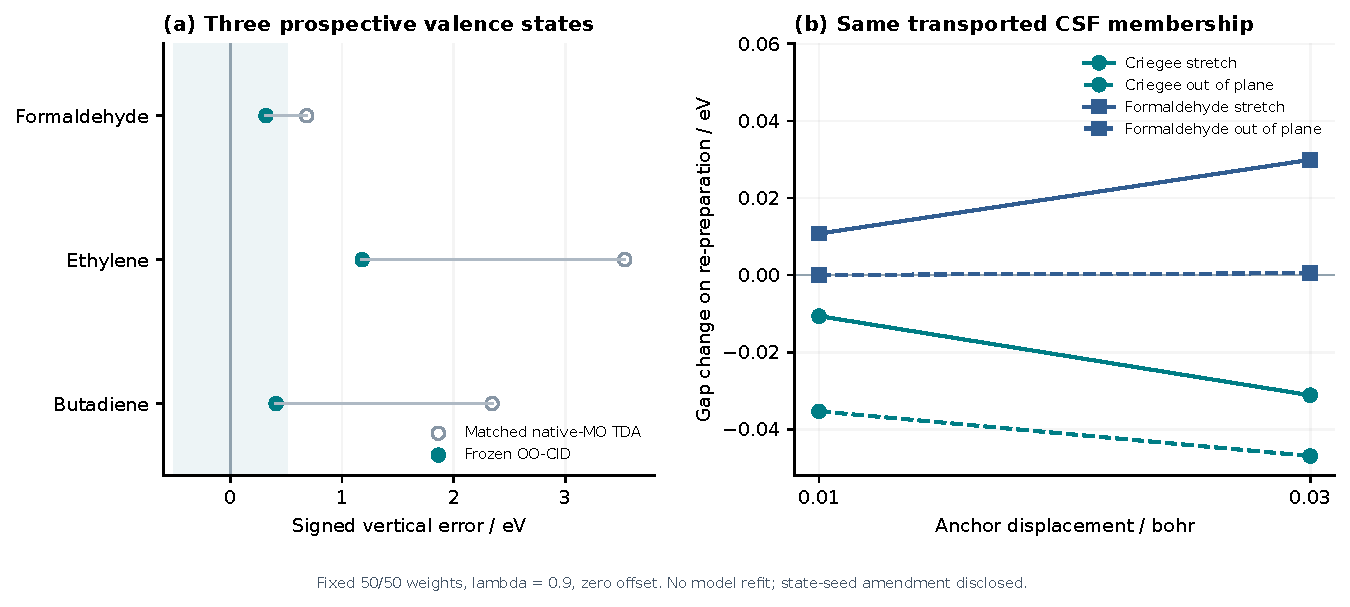
\includegraphics[width=\linewidth]{figures/closing_validation.pdf}
\caption{Final prospective extension and reference-geometry sensitivity.
(a) OO-CID and matched native-orbital TDA signed errors for every new state;
the shaded region is $\pm0.5$ eV. (b) Re-prepared versus original-anchor
excitation gaps evaluated at identical displaced geometries, with the
original CSF membership transported by occupied/virtual orbital overlap.
The model parameters are unchanged. The small extension is separate from
the exposed twenty-state development set.}\label{fig:closingvalidation}
\end{figure}

Anchor tests displace one carbon by 0.01 and 0.03 bohr in an in-plane
stretch or an out-of-plane direction, for the Criegee intermediate and
formaldehyde. Each comparison uses the same physical final geometry,
retains all originally prepared target states and reuses the completed
reference checkpoints. With the original CSF membership transported by
orbital overlap, the largest gap change is 0.047 eV for the Criegee
$\pi\pi^*$ state and 0.030 eV for formaldehyde. These are local controls,
not a bound on arbitrary anchor displacement. Re-selecting the configuration
space at each new anchor is a different operation: loss of the Criegee
reflection certificate reduces its space from 178 to 13 CSFs and changes
the $\pi\pi^*$ gap by 0.263--0.273 eV. A trajectory must retain its frozen
chart; symmetry-dependent space selection must not be silently reapplied
at every displaced geometry. The implemented analytic surface already
retains this membership during nuclear motion.

\subsection{Predecessor structures, frequencies and exact acceleration}
The frozen screened-even predecessor was optimized on the lowest singlet surfaces of
formaldehyde and acetaldehyde using analytic gradients. Full analytic
Hessians then assess the vibrational curvatures. Coupled-cluster internal
coordinates provide a physical structural comparison,\cite{geometries2017}
and selected experimental vibrational fundamentals provide a separately
identified spectroscopic comparison.\cite{formaldehydespectrum1969,acetaldehydespectrum1981}
The model frequencies are unscaled harmonic curvatures, whereas the
experimental numbers are anharmonic level spacings. Modes are assigned
through projections on mass-weighted chemical-coordinate displacement
patterns, rather than matched by frequency order. Inversion splittings and
methyl-torsion level spacings are not used as harmonic curvature references.
Complete coordinates, modes and individual differences are given in the
Supporting Information. These comparisons assess that predecessor energy;
they are not substituted for equilibrium data of the subsequently corrected reference.

A further exact response optimization vectorizes the overlap-residual
completion and avoids scalar derivative-jet allocation for frozen
auxiliary matrix values. A cold two-thread Criegee public-API Hessian takes
397 s, compared with the archived 418 s; energies, gradients and both full
Hessians are bitwise identical between versions. Peak resident memory is
1.19 GB, compared with 1.06 GB. This single-run 4.9\% time reduction is
modest, with other work active on the host, and is not evidence of a
size-scaling improvement or a speed advantage over TDA. The ten algebra,
spin and legacy-contract regressions also pass. No numerical derivative,
Hamiltonian change or fitted correction enters the acceleration.

\subsection{Resolving the ethylene extension with a common screened reference}
The prospective ethylene discrepancy motivates a second, separately
identified development candidate. The F reference represents the full DFT
Fock operator in a confined valence image, whereas its qualified Q levels
come from the larger DFT calculation. To assess this imbalance, let $P$
be the isometric native-valence image and $Q$ its orthogonal complement
in the complete DFT orbital space. For an already qualified orbital match,
we evaluate the diagonal complement self-energy
\begin{equation}
 \Sigma_i(E_i)=F_{iQ}(E_i-F_{QQ})^{-1}F_{Qi}
\end{equation}
at its matched DFT orbital energy and add it to the F level before the
unchanged 50/50 average. Unqualified matches retain their original reference.
This is a diagonal downfolding approximation, not an exact many-electron
elimination of the DFT environment. No excitation reference enters this
one-body preparation. It lowers the ethylene result from 9.079 to 8.206 eV,
consistent with a substantial confinement contribution to the initial error.

The environment screening is rebuilt using Coulomb vertices between native
occupied orbitals and an explicit orthogonal DFT bath, avoiding the use of
missing active-orbital spectral weight as an independent screening channel.
Subspace disentanglement is a recognized issue in constrained
screening.\cite{miyake2009} We allow one global semiempirical efficiency
$\eta$ for this additional bath polarization:
\begin{equation}
 W=L_P^\mathrm{T}
 \left[I+B_NB_N^\mathrm{T}+\eta B_BB_B^\mathrm{T}\right]^{-1}L_P .
\end{equation}
Here $B_N$ contains the retained native environment transitions, $B_B$
the occupied--bath transitions, and $L_P$ the native Coulomb vertices.
The one-body interaction is normal ordered to the corrected native ground
Fock. The retained configuration space is unchanged. Static screening is
an approximation whose quantitative limitations also arise in molecular
RPA downfolding.\cite{verzijl2026}

We calibrate $\eta=0.60$ by balancing the opposite errors of furan V010
and furofuran C002, and freeze it before evaluating the complete ledger.
This is \emph{one fitted interaction parameter}; it is neither an energy
offset nor a parameter-free correction. It applies to every molecule and
state. The F/Q weights stay 50/50, exchange-response $\lambda$ stays 0.9,
and orbital gaps are not multiplied by either parameter. All 23 numerical
labels have been exposed during development, including the three-state
extension, so this assessment is not a blind validation.

\begin{figure}[!htbp]
\centering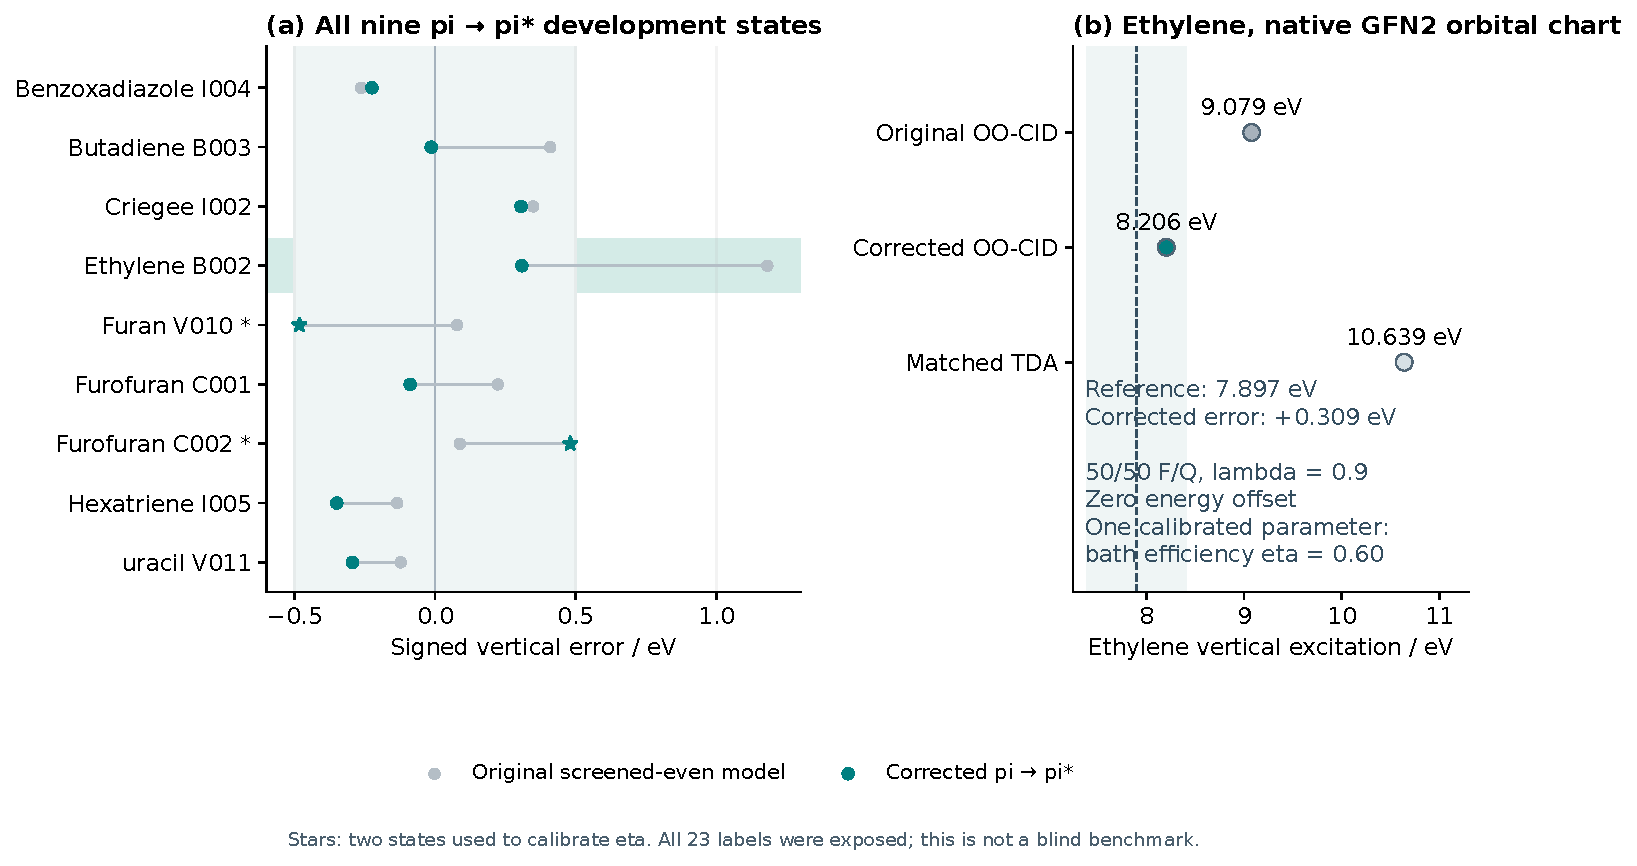
\includegraphics[width=\linewidth]{figures/ethylene_repair.pdf}
\caption{Common-reference repair on the complete exposed development set.
(a) Original and corrected signed errors for all nine $\pi\pi^*$ states; stars identify
the two states used to calibrate bath efficiency $\eta$. (b) Ethylene's
initial and corrected OO-CID energies, with a freshly evaluated TDA control
using the corrected native GFN2 ground orbitals and reference response.
The reference is 7.897 eV. The shaded intervals are $\pm0.5$ eV.}
\label{fig:ethylenerepair}
\end{figure}

All nine $\pi\pi^*$ states now lie within 0.5 eV, with MAE 0.283 eV and
maximum error 0.482 eV. The fourteen $n\pi^*$ states give 0.175 eV MAE
and 0.381 eV maximum error. All 23 states give 0.217 eV MAE. The 21 states
not used to choose $\eta$ give 0.192 eV MAE; their earlier exposure still
precludes a blind-validation claim. The matched corrected-reference TDA
MAEs are 1.726 eV for $\pi\pi^*$, 0.174 eV for $n\pi^*$ and 0.781 eV
overall. Thus the measured accuracy benefit is concentrated in $\pi\pi^*$;
the two $n\pi^*$ mean errors are essentially equal. This response control
is not a separately optimized published TDA parameterization.

Ethylene has error $+0.309$ eV. Its full analytic Hessian takes 10.15 s on
the verified two-thread Mac Studio run; two independent scalar-energy
Richardson checks give maximum errors $1.73\times10^{-11}$ Ha/bohr for
the gradient and $6.56\times10^{-8}$ Ha/bohr$^2$ for directional curvature.
The coherent singlet has $\langle S^2\rangle=0$, and its accepted restart
agrees within $8.9\times10^{-16}$ Ha. No DFT import, TDA solve or new SCC
driver is used during prepared evaluation. These derivatives belong to the
corrected frozen anchored surface. The earlier minimum and frequency
comparisons in the preceding subsection belong to its screened-even
predecessor and are not reassigned to this calibrated extension. Independent
prospective molecules and corrected-model equilibrium structures remain
necessary before a general transferability claim.

\subsection{Fragmented orbital matches and three further valence tests}
The fixed $\eta=0.60$ candidate is next applied to cyclopropene,
cyclopentadiene, and pyrrole. All three predictions are archived before
extracting their numerical QUEST references. Their errors are initially
$+0.054$, $-0.013$, and $+2.369$ eV. Historical exposure of some of these
molecules prevents a strictly blind claim. Pyrrole's discrepancy exposes
a reference-construction limitation: its native virtual orbitals have
substantial weight distributed over several full-DFT virtual orbitals,
so no individual match meets the existing 0.7 amplitude criterion.
The original fallback therefore omits both the qualified Q level and the
complement relaxation for these orbitals.

We amend this rule for \emph{every} unresolved occupied or virtual orbital,
without a molecule or state-family branch. Within the same occupation
sector, full-DFT poles are ordered by native spectral weight $w_{ki}$.
The smallest block $\mathcal B_i$ satisfying
$\sum_{k\in\mathcal B_i}w_{ki}\geq0.7^2$ supplies the normalized centroid
\begin{equation}
 \mu_i=\frac{\sum_{k\in\mathcal B_i}w_{ki}\epsilon_k}
 {\sum_{k\in\mathcal B_i}w_{ki}} .
\end{equation}
This centroid supplies the Q level with the original occupied-centroid
alignment. Its difference from the Rayleigh energy of the original
native image supplies the unresolved F relaxation. Individually qualified
poles retain their preceding treatment. We then rebuild the explicit
bath screening on the corrected native orbitals. The 50/50 average,
$\lambda=0.9$, $\eta=0.60$, configuration rule and zero energy offset remain
fixed. This is a diagonal spectral-centroid approximation, not an exact
elimination of a broad or frequency-dependent environment. The reference
preparer reads no excitation labels, but the amendment was developed after
pyrrole scoring: the resulting ledger is an exposed development assessment.

Pyrrole then gives 6.302 eV against 6.247 eV. Applying the identical rule
to all 26 states in 24 molecules gives MAE 0.198 eV and maximum error
0.446 eV. The twelve $\pi\pi^*$ states give 0.216 eV MAE; the fourteen
$n\pi^*$ states give 0.183 eV. All individual errors are below 0.5 eV.
Matched TDA on the corrected native GFN2 orbitals gives 0.789 eV MAE
overall, 1.514 eV for $\pi\pi^*$ and 0.168 eV for $n\pi^*$: the OO gain
is concentrated in the $\pi\pi^*$ family, while TDA has the smaller mean
$n\pi^*$ error. Neither comparison is a calibrated sTDA-xTB benchmark.
Every prepared state passes fresh-process spin and restart checks with no
DFT import, new SCC call or TDA solve. Ethylene's updated full analytic
Hessian takes 10.68 s; scalar-energy Richardson checks give errors below
$9.92\times10^{-12}$ Ha/bohr and $2.46\times10^{-8}$ Ha/bohr$^2$.
These remain derivatives of a frozen anchored model.

\begin{figure}[!htbp]\centering
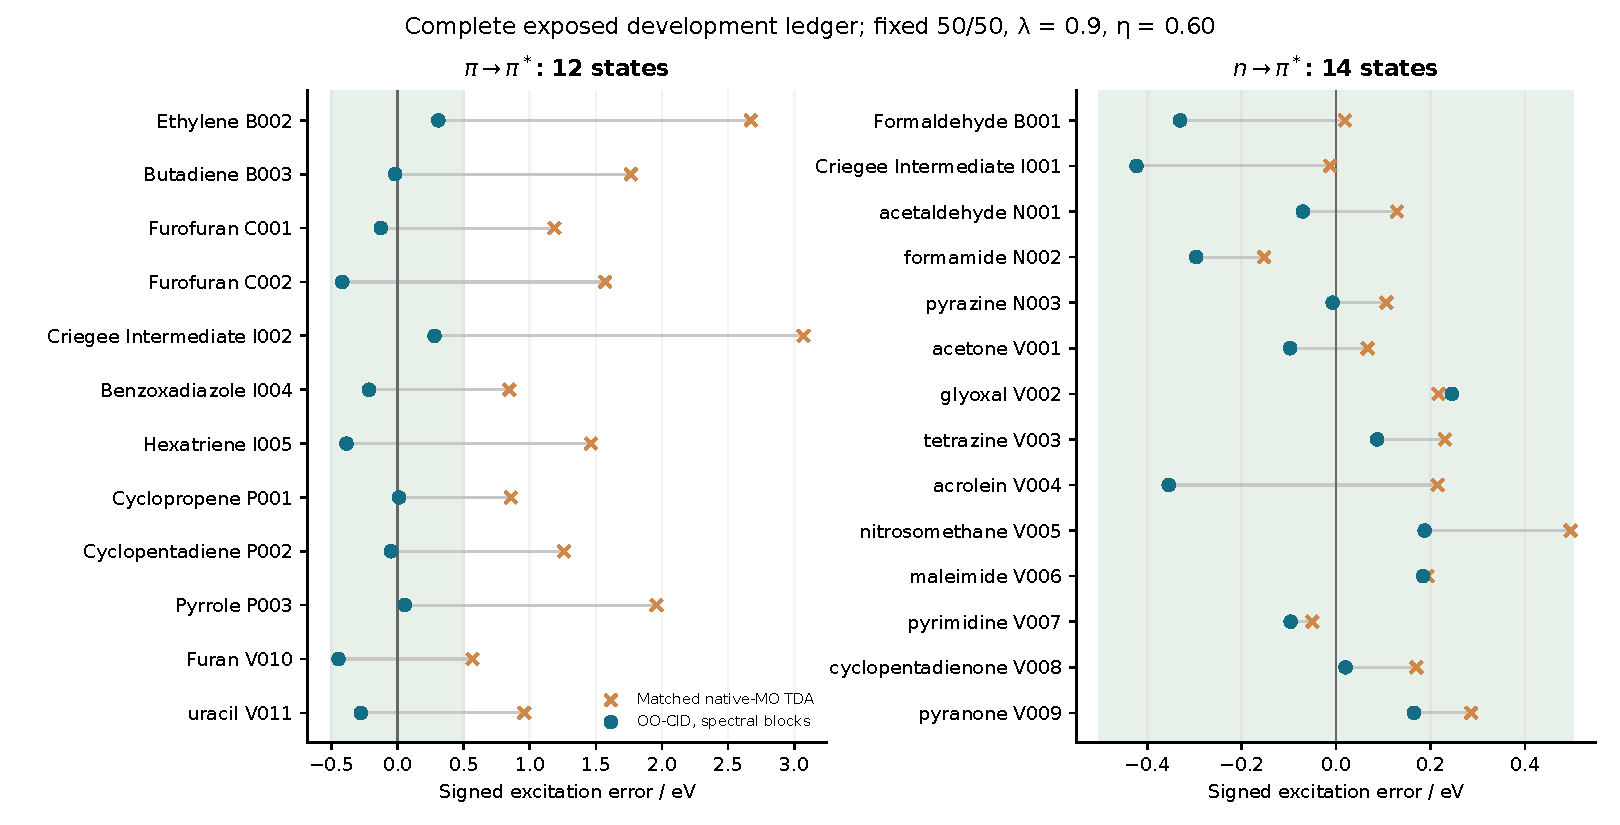
\includegraphics[width=\linewidth]{figures/spectral_block_validation.pdf}
\caption{All 26 exposed development states after the generic spectral-block
reference amendment. Points compare OO-CID with freshly calculated TDA on
the same corrected native orbitals. The shaded interval is $\pm0.5$ eV.
The two panels use different horizontal scales. Neither the bath efficiency
nor the F/Q weights are retuned for the three added molecules.}
\label{fig:spectralblocks}
\end{figure}

\subsection{Matrix-free orbital response for larger valence spaces}
For the pigment examples, the constrained ROKS orbital residual is solved
by Newton--Krylov iterations. An analytic Jacobian action differentiates the
native Fock and spin response, the orbital rotations, and the determinant
ground-overlap constraint. The covariant orbital action is symmetric; the
ground constraint is differentiated with singular-safe determinant
cofactors. No dense orbital Jacobian is allocated and no finite difference
enters the production orbital solver. All nonredundant orbital rotations
are retained. A residual-decreasing line search controls each accepted
step, while checkpointed overlap tracking follows the coherent singlet
between accepted steps. Its character relative to the initial transition
is reported separately. Final CI targets are assigned by collective
overlap with the frozen native-frontier singlet subspace; this allows
mixed frontier excitations without identifying a state by its energy.
When a target fragments over several CI eigenstates, roots are retained
until the smallest eigenvalue of their projector in the fixed target space
reaches 0.49. This keeps the original coverage threshold, protects each
target direction and is invariant to unitary rotations of the target basis.

A direct-energy initialization precedes the final KKT search when a
residual-norm minimization stagnates. The promoted open orbitals are
first held fixed while L-BFGS relaxes the remaining orbitals. Analytic
exponential-map pullbacks provide the optimization gradient. Ground
orthogonality is enforced through an augmented Lagrangian,
$E_{\rm ROKS}-\mu o+\kappa o^2/2$, with multiplier updates
$\mu\leftarrow\mu-\kappa o$. This is a numerical constraint objective;
the penalty is excluded from reported energies. All nonredundant
rotations are subsequently released and the original full-functional
KKT equations determine convergence. This freeze-and-release sequence
is motivated by the direct-optimization strategy of Levi and
co-workers.\cite{freeze2026} A second converged root is distinguished
from an existing solution by its coherent singlet overlap. If two
frontier promotions collapse onto the same root, a new initial hole
is chosen as the orthogonal complement of the converged hole within
the same frozen native frontier block. This changes the initial guess,
not the energy model or the final stationarity equations.

The large-system XC response is evaluated on its full frozen quadrature.
A density-fitted approximation preconditions the Newton linear system.
When its step fails the full-response inexact-Newton tolerance, flexible
GMRES refines it with analytic full-quadrature Hessian actions. The
ground-constraint factorization is cached within each linear solve.
The moving-frame Jacobian is also available to GMRES by subtracting the
analytic skew connection from the covariant action. The physical orbital
Hessian remains the symmetric covariant response. A Newton step that
already exceeds the trust radius need not be refined before the bounded
subspace problem; its full-response descent direction and predicted
reduction are still evaluated explicitly. For
large Newton steps, a residual-minimizing trust subspace contains the
Newton and full-response squared-residual descent directions, augmented
by directions retained from the auxiliary Krylov solve. Twice-applied
orthogonalization removes redundant directions. When retraction is enabled, every orbital basis direction is first
projected to satisfy $\mathbf j^{\mathsf T}\delta\boldsymbol\theta=0$.
The small constrained least-squares problem bounds the orbital rotation;
the unrestricted multiplier is eliminated exactly by projection in the
residual space. A thin singular-value decomposition of the response
images solves the trust problem directly. Normal equations would square
the condition number and could discard physically relevant soft modes.
The predicted reduction therefore describes the same tangent step that
the subsequent geometric retraction executes. The auxiliary response can
propose an enlarged-subspace step; its predicted reduction is then
recomputed with the full quadrature action, and acceptance requires an
actual decrease of the full functional residual. The trust radius adapts
to the ratio of actual and predicted squared-residual reduction. This
avoids excessively small steps along soft orbital modes without changing
the energy or stationarity equations. The adapted radius is saved with
the accepted orbital checkpoint and restored on continuation.
For the constrained search, each trial can additionally be retracted onto
the original zero ground-overlap manifold by short orbital rotations
along its analytic cofactor gradient. No energy evaluation enters this
geometric correction. At fixed trial orbitals the scalar multiplier is
eliminated by least squares, $\mu=(\mathbf j^{\mathsf T}\mathbf g)/
(\mathbf j^{\mathsf T}\mathbf j)$ when the constraint gradient
$\mathbf j$ is nonzero. The full KKT residual, including the overlap,
remains the convergence criterion. This avoids rejecting an otherwise
useful tangent step solely because its finite rotation creates a
second-order overlap; it does not replace ROKS by a projected energy.
Writing $a=c,s$ for charge and spin channels, the actual energy is
\begin{equation}
 E=E_{\mathrm{RI}}+\frac12\sum_a
 \left[\int \delta\bm\rho_a(\mathbf r)^{\mathsf T}
 f_{\mathrm{xc},a}(\mathbf r)\delta\bm\rho_a(\mathbf r)\,d\mathbf r
 -\mathbf q_a^{\mathsf T}K_{\mathrm{xc},a}^{\mathrm{RI}}\mathbf q_a\right],
\end{equation}
where $\bm\rho$ contains the density and its three Cartesian derivatives.
The charge deviation is measured from the anchored native ground density;
the spin deviation is the spin density itself. Thus the approximate XC
quadratic form is subtracted and the full quadrature form restored in
both the energy and the convergence residual. Stored basis values,
quadrature weights and XC kernels suffice for evaluation without a DFT
backend. On ethylene, energy, Fock and response equivalence errors are
below $2.5\times10^{-15}$ in the corresponding atomic units; the spin-pure
CI matrix agrees within $3.6\times10^{-15}$ Ha. These controls distinguish
an acceleration of the stationarity search from a change of energy model.

CI assembly likewise preserves the Hamiltonian while avoiding a full
four-index molecular-orbital transformation: the common closed-shell core
is contracted first and only the active integral block is transformed.
Fixed-bra Schur contractions reuse the common core in nonorthogonal
couplings; repeated identical canonical occupations reuse their exact
cofactors and pair contractions through a bounded cache. Retained-CSF
transition-density actions are batched into exact matrix products; identically
zero second cofactors bypass their pair-tensor contraction. Canonical columns
with a common retained bra are evaluated in batches with the same determinant
cofactors and spin coefficients. Their active/null pair features remain outer
products: the auxiliary factors are transformed along the two orbital indices
before contraction, avoiding a flattened dense feature transform. Division-free prefix/suffix
products form the first and second spectral cofactors while retaining
multiple zero singular values. Coulomb
feature contractions use the existing auxiliary factors of the same
screened interaction, with no additional fitting or truncation. The canonical
determinant-to-CSF transformation uses its exact sparse coefficients
instead of dense multiplication; no determinant or spin coupling is
dropped. An optional Numba-compiled integer-mask Slater--Condon loop
retains the Python reference implementation; it uses neither fast-math
nor integral screening. Independent tests, including the highest bit of
a 64-spin-orbital mask, agree within $2.1\times10^{-13}$ Ha.
Singular cofactors are evaluated as products of the remaining
singular values without division. Registered density spans accelerate the
quadratic native energy only when the requested density lies in that span;
otherwise evaluation falls back to the full expression.
Frontier records are enumerated directly from at most two occupied holes
and two virtual particles, in $O(N^4)$ operations, instead of generating
and rejecting higher-rank occupations. The canonical block is retained
as dense arrays rather than a dictionary of scalar pairs. Identical
nonorthogonal matrix elements can be reused between nested windows only
when their model, screening and orbital identities match exactly.
Ground-state removal is an exact rank-one projection. Generalized
Lanczos iterations use a sparse metric inverse and its exact rank-one
Sherman--Morrison update; only the requested roots are returned, without
reducing the configuration space. On the archived 2,145-CSF problem,
the lowest twenty energies reproduce the full dense solution within
$2.0\times10^{-12}$ eV, with residuals below $1.5\times10^{-13}$ Ha.
Observable contractions use exactly the determinant ordering of the
Hamiltonian. Phase tests cover even and odd occupations and direct
overlaps with the stored metric. Identical native diagonal and four-spin
functional values can be reused when only the screened interaction
changes; an independent matrix reconstruction agrees within
$2.0\times10^{-11}$ Ha for the archived carotene block and
$1.1\times10^{-10}$ Ha for chlorophyllide. The 45 retained-CSF scalar
elements of chlorophyllide reproduce the unbatched journal within
$1.9\times10^{-12}$ Ha. Batched reconstruction of the 3,406-CSF
chlorophyllide pencil at $N=W=9$ agrees with the saved matrix within
$6.9\times10^{-13}$ Ha. Positive definiteness is certified by a Gershgorin lower bound or by
eliminating the sparse canonical block and testing its small border
Schur complement. A smallest-eigenvalue calculation remains the fallback.


Native real d functions are included in the molecular-frame transport
with analytic first and second rotation derivatives. Large-system native
response also uses the same D4 and electrostatic cutoffs as its ground
functional. Dense pair tensors and screened interactions are still stored:
matrix-free orbital stationarity does not make this implementation
linear-scaling or inexpensive in memory. The present quadrature adapter
supports vertical energies and orbital response only; it explicitly rejects
nuclear-derivative requests. The analytic nuclear Hessian qualifications
reported for the small-molecule anchored surface therefore do not extend
to these pigment calculations.

\paragraph{Coherent transition constraints in the pigment screening test.}
A product of separately enlarged hole and particle spaces generally exceeds
its explicit CI transition space. At $N=16$, the former contains 400 native
response directions for chlorophyllide, whereas the actual canonical-single
and optimized-CSF one-body amplitudes span 257 directions. The corresponding
numbers for carotene at $N=13$ are 196 and 169. This over-exclusion removes
polarization channels that the explicit configurations do not restore.
We therefore test a general correction using the actual transition amplitudes.
Let $D$ contain the positive native orbital gaps, let $L$ be the native
Coulomb vertices, and let $A$ collect the canonical-single coordinate vectors
and the exact one-body transition amplitudes of the retained optimized CSFs.
With $B=2LD^{-1/2}$ and $U$ an orthonormal basis for $D^{-1/2}A$, the
constrained native polarization is
\begin{equation}
 \Pi_{\rm n}=B(I-UU^{\mathsf T})B^{\mathsf T}.
\end{equation}
This is the response of the positive quadratic resolvent under the coherent
constraints, rather than a diagonal probability mask. Canonical directions
are removed directly; a thin SVD resolves the remaining optimized-CSF
columns. The orthogonal DFT bath, $\eta=0.60$, F/Q weights, exchange scale,
native functional and converged ROKS checkpoints are unchanged. No excitation
energy enters the construction. The earlier product-space sequence and the
corrected transition-space sequence are retained as separate model generations;
the pigment extension is not pooled with the 26-state exposed accuracy ledger.
The new projector is checked against the direct constrained inverse and under
unitary changes of its active basis. Screening and all CI matrices are frozen
within each fixed-interaction convergence sequence.

The canonical accelerator also supports two-word, 128-bit spin-orbital
masks. Fermionic parity includes both words, and the sparse
determinant-to-CSF transform is contracted during Slater--Condon assembly.
This avoids allocating the dense determinant Hamiltonian when extending
beyond 32 active spatial orbitals. Tests cross the 64-bit boundary and
compare with arbitrary-precision occupation algebra. The common-core
cofactor accelerator supports up to 32 active electrons per spin without
changing its determinant polynomial. Native functional diagonals and
four-spin blocks from a smaller completed frontier are reused after model,
orbital and record-identity checks; screened couplings are recomputed when
the screening partition changes.

For the static-matched candidate, an optional generalized block Davidson
solver reuses the stored CI subspace. Rank-revealing metric orthogonalization
handles the dependent residual directions produced by a low-rank Hamiltonian
update. Only redundant search directions are removed; all configurations
and matrix elements remain in the operator. Row-block matrix products can
share the immutable Hamiltonian across workers. Every returned root must
pass the full generalized residual and metric-normalization tests. This
algorithm changes the numerical search, rather than the physical model.

The Davidson metric action chooses sparse or dense storage from the exact
nonzero density. Dense metrics use matrix multiplication directly;
small nonzero entries are retained without thresholding. This avoids a
serial sparse-multiplication bottleneck when ground projection produces
a dense metric. The choice changes storage and execution only, leaving
the generalized pencil and residual tolerance unchanged.


\subsection{Larger pigment structures and a carotene vertical example}
We select all-trans $\beta$-carotene and chlorophyllide a as larger
chromophore tests. Chlorophyllide a retains Mg and the conjugated
substituents while removing the phytyl chain. Figure~\ref{fig:pigmentstructures}
shows the actual source structures, rather than schematic molecular art.
Native ground checkpoints contain 216 and 219 orbitals, respectively.
The chlorophyllide reconstruction explicitly includes Mg d functions.
Raw Gaussian-overlap discrepancies and subsequent numerical metric
reconciliation are archived separately; agreement after reconciliation is
$2.5\times10^{-13}$ or better. The one-time PBE0/CAM-B3LYP reference
preparation uses checkpointed RI-JK calculations on the verified Mac Studio.
The carotene ROKS target converges at 3.518 eV, with orbital KKT residual
$4.73\times10^{-12}$ and ground-CSF overlap $1.32\times10^{-13}$.
The initial 15-CSF screened-CID space incorrectly places an intense state
at 3.269 eV below a weak state at 3.680 eV. We therefore expand the native
frontier window with all spin-singlet configurations of excitation rank
at most two, retaining the optimized ROKS configurations. The F/Q weights,
$\lambda$, $\eta$, geometry and zero offset remain fixed. The resulting
15, 153, 351 and 703-CSF calculations are retained in the
Supporting Information, including the initial ordering.

With five occupied and five virtual frontier orbitals, the first state
becomes weak at 2.561 eV, followed by an intense state at 2.728 eV. This initial ordering repair motivates further
configuration-space checks rather than an absolute-energy convergence claim.

The screening window $W$ defines the native transitions excluded from
polarization; it is an active partition, not a numerical polarization cutoff.
For the final sequence we set $W=N$, matching the represented canonical
CI frontier and its polarization exclusion. At fixed $N$, increasing $W$
removes additional response channels without adding their CI configurations
and changes the effective model. Such sensitivity checks are retained
separately in the Supporting Information.

We require the first three ordered gaps to change by less than 0.02 eV
in each of two consecutive frontier increments. The coherent $W=N$
sequence uses 7,503, 10,585 and 14,535 CSFs at $N=11,12,13$
(Figure~\ref{fig:carotenespace}). At $N=13$, the three gaps are
1.950, 2.338 and 2.478 eV, with oscillator strengths 0.00117,
0.132 and 4.796. The largest change across either final increment is
0.0054 eV. The lowest state remains weak and the dominant intensity
belongs to the third energy-ordered state.

An independent fixed-Hamiltonian check at $W=16$, with the same three
CI windows, gives a maximum increment of 0.0021 eV. Nested principal
blocks agree within $7.7\times10^{-13}$ Ha, their metrics within
$6.8\times10^{-15}$, and the ground energies are identical. The final
squared principal cosines of the roots 2--3 subspace exceed 0.9998.
Numerical dielectric residuals are below $3.4\times10^{-15}$.
These tests establish frontier convergence at the stated tolerance for
the prepared rank-two model, with unchanged geometry, F/Q weights,
$\lambda$, $\eta$ and zero energy offset.

The development sequence also illustrates target fragmentation. At
$N=9$, $W=10$, roots 2 and 3 carry individual native-target weights
0.420 and 0.385 but joint coverage 0.805. Collective target tracking
retains this resolved mixed subspace without changing the Hamiltonian.
Energy indices and bright character must be distinguished through mixing.
The full window sequence and transition strengths are archived in the
Supporting Information.

The first state is weak rather than strictly forbidden on the unoptimized
source geometry. Room-temperature fluorescence-derived $S_1$ energies
and solvent absorption maxima are different observables and cannot
validate these vertical gaps directly. The known low-lying dark state
motivates the expanded configuration space~\cite{Bondarev1994}; pigment
absorption data provide experimental context~\cite{Clementson2019}.
The expansion follows exposure of the spectra and is a development test,
not blind validation. The four chlorophyllide frontier targets now give distinct stationary
ROKS solutions with maximum residual $3.5\times10^{-11}$ and a smallest
singlet-overlap eigenvalue of 0.688. Direct-energy freeze-and-release
initialization removes the residual-norm stagnation; the Supporting
Information gives the unshifted ROKS energies and the root-identity audit.
These stationary basis states precede the final screened-CID calculation;
a correlated chlorophyllide spectrum is not claimed here.
Both pigments remain excluded from the 26-state accuracy pool; neither
excited minima nor pigment nuclear Hessians are reported.

\begin{figure}[!htbp]\centering
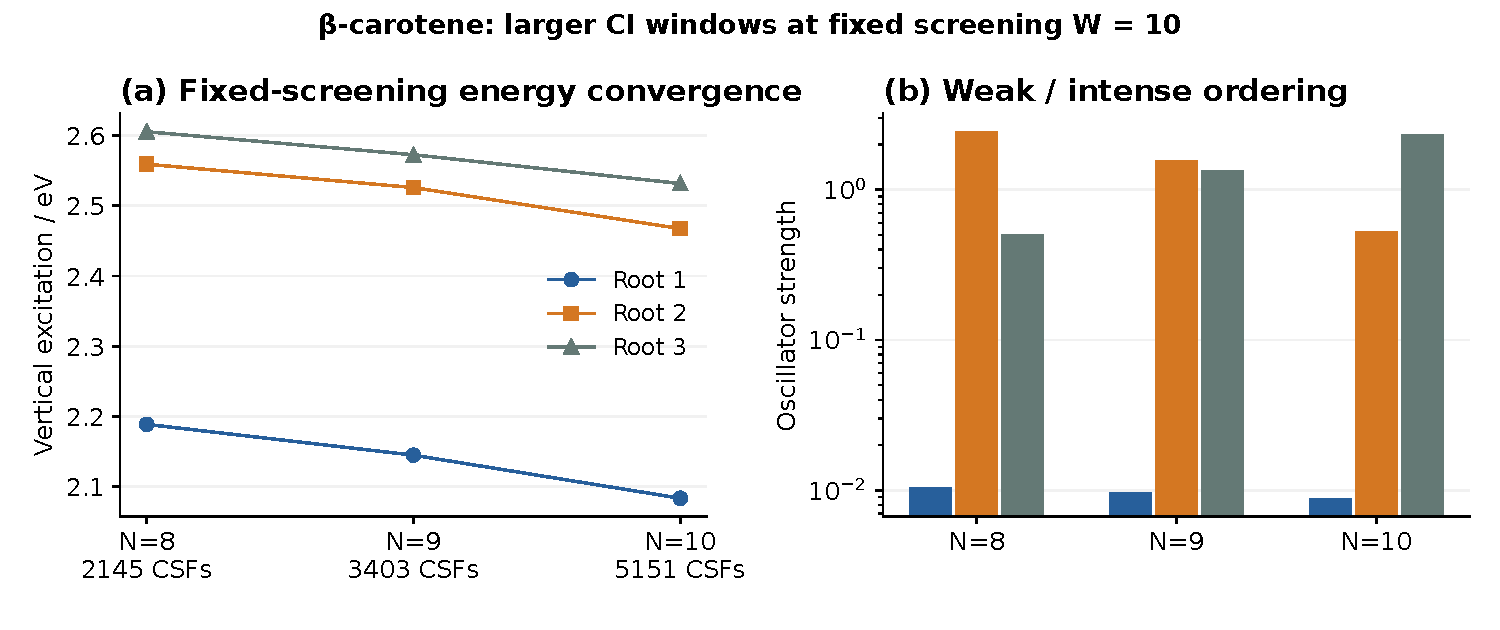
\includegraphics[width=\linewidth]{figures/beta_carotene_convergence.pdf}
\caption{Convergence of $\beta$-carotene with 11--13 occupied and virtual
frontier orbitals. Solid lines use matched CI and polarization exclusion
($W=N$); dashed lines show the independent fixed-Hamiltonian check
at $W=16$. Bars show the coherent-window oscillator strengths.
The weak first singlet lies below an absorbing pair, with the dominant
intensity on root 3. Lines connect energy-ordered roots; subspace overlaps
are tracked separately. Parameters and source geometry remain fixed.
The initial 15--703 CSF ordering repair is retained in the Supporting Information.}
\label{fig:carotenespace}
\end{figure}

\begin{figure}[p]\centering
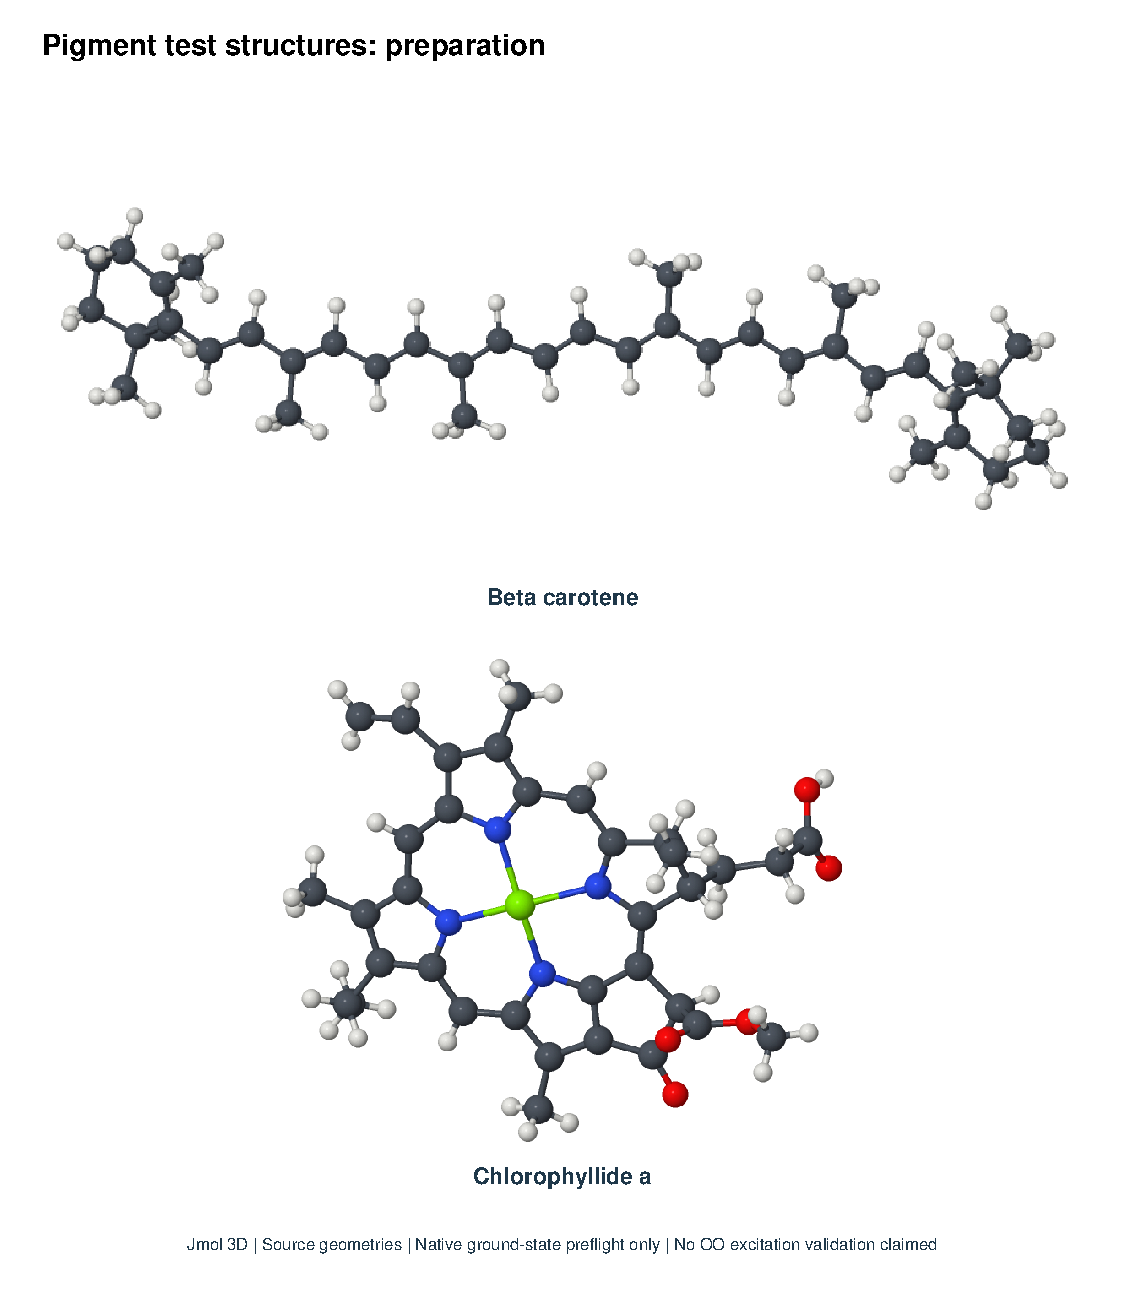
\includegraphics[width=.92\linewidth,height=.80\textheight,keepaspectratio]{figures/pigment_test_structures_jmol.pdf}
\caption{Jmol renderings of the larger starting structures: all-trans
$\beta$-carotene (96 atoms; PubChem CID 5280489) and chlorophyllide a
(79 atoms; RCSB ligand A1JWG). These primary-source geometries are used
for preparation and are not optimized excited-state structures or
validated additions to the accuracy ledger.}
\label{fig:pigmentstructures}
\end{figure}

\subsection{Static matching of the extended configuration interaction}
Adding explicit configuration interaction to density-functional diagonal
energies requires deciding which correlation is already represented.
DFT/MRCI addresses this
issue through an effective Hamiltonian with empirical damping.\cite{marian2019mrci}
We examine zero-frequency self-energy subtraction, following its use in
extended response theories.\cite{tselyaev2013,gambacurta2015}
The borrowed principle is static matching. Its molecular OO-CID application
is a development proposal, rather than an exact density-functional result.

After removing the native ground CSF, define
$\widetilde H=P_g^\dagger(H-E_gS)P_g$ and
$\widetilde S=P_g^\dagger SP_g$. The fixed primary space contains the
optimized singlets and their paired partners; the complementary space
contains all canonical auxiliary configurations. Metric orthogonalization
of the latter gives
\begin{align}
 X&=\widetilde S_{PP}^{-1}\widetilde S_{PQ},\qquad
 A=\widetilde H_{PP},\qquad V=\widetilde H_{PQ}-AX,\\
 D&=\widetilde H_{QQ}-\widetilde H_{QP}X
       -X^\dagger\widetilde H_{PQ}+X^\dagger AX.
\end{align}
Adding $VD^{-1}V^\dagger$ to the primary block in these coordinates yields
\begin{equation}
 H_{\mathrm{eff}}^{\mathrm{sub}}(\omega)
 =A+VD^{-1}V^\dagger+V(\omega S_Q-D)^{-1}V^\dagger,
 \qquad H_{\mathrm{eff}}^{\mathrm{sub}}(0)=A ,
\end{equation}
where $S_Q=\widetilde S_{QQ}-\widetilde S_{QP}X$.
The complete interacting $D$ is used, rather than its diagonal. Its
positivity is checked before inversion. No damping coefficient, constant
excitation shift or orbital-reference adjustment is fitted. The 50/50
weights, $\lambda=0.9$ and previously calibrated $\eta=0.60$ are unchanged.

On the same 26 exposed states, the MAE changes from 0.198 to 0.183 eV.
The $\pi\pi^*$ and $n\pi^*$ MAEs become 0.209 and 0.160 eV. The maximum
individual error increases from 0.446 to 0.478 eV; all errors remain
below 0.5 eV. Table~\ref{tab:staticmatching} and
Figure~\ref{fig:staticmatching} show both the mean improvement and the
cases that become less accurate. All 24 models reproduce these energies
through the public API, with coherent-singlet spin and accepted-restart
checks. These exposed labels do not provide independent transferability
validation.
\begin{table}[!htbp]\centering\small
\caption{Static-matching development candidate on the same corrected native orbitals, geometries and 26 exposed reference labels. No parameter is refitted. All errors are in eV.}
\label{tab:staticmatching}
\begin{tabular}{lrrrrr}\toprule
Family & States & TDA MAE & Before MAE & Matched MAE & Matched max.\\\midrule
All & 26 & 0.789 & 0.198 & 0.183 & 0.478\\
$\pi\pi^*$ & 12 & 1.514 & 0.216 & 0.209 & 0.478\\
$n\pi^*$ & 14 & 0.168 & 0.183 & 0.160 & 0.411\\
\bottomrule\end{tabular}
\end{table}

\begin{figure}[!htbp]\centering
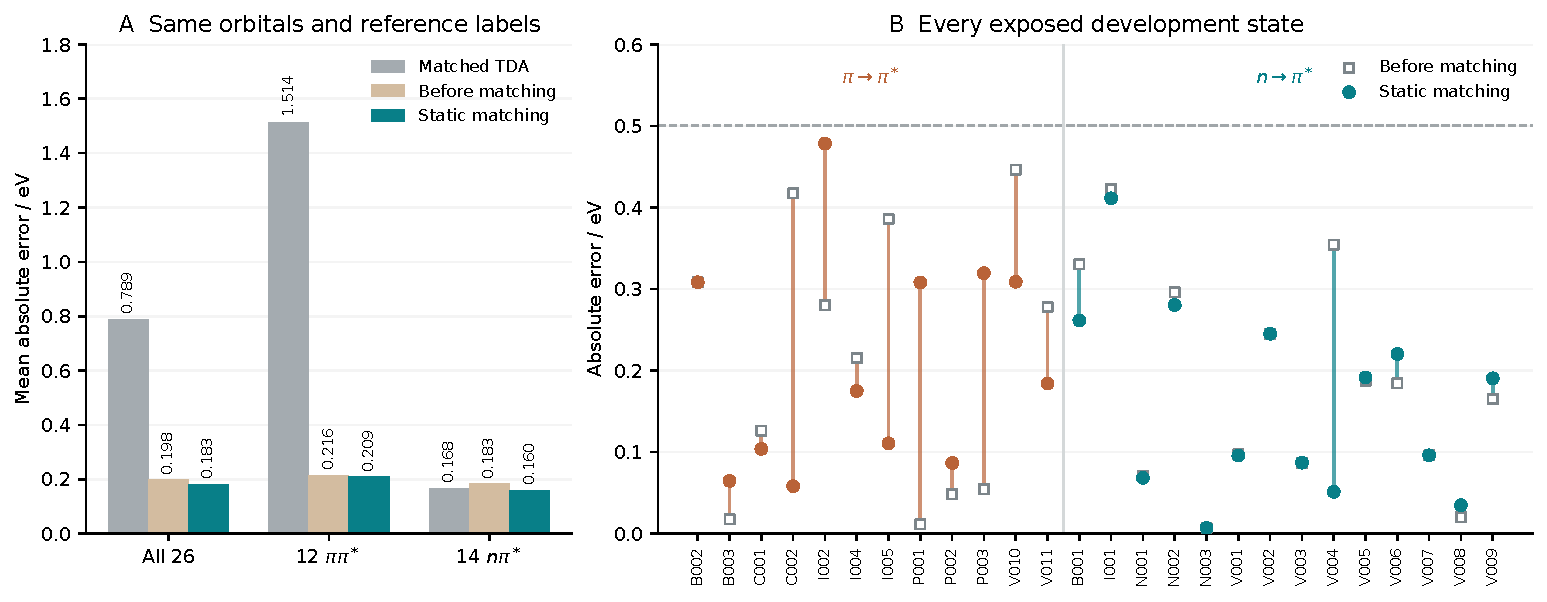
\includegraphics[width=\linewidth]{figures/static_subtraction_accuracy.pdf}
\caption{Static matching on the unchanged exposed development set.
(A) Family-resolved MAEs compared with the unsubtracted candidate and
matched TDA on the same corrected native GFN2 orbitals. (B) Every individual
absolute error before and after matching. The dashed line marks 0.5 eV.
No parameter is refitted and no molecule or state-family branch is added.
This is a development comparison rather than blind validation.}
\label{fig:staticmatching}
\end{figure}

The counterterm participates in the complete analytic nuclear response.
Both derivatives of $D^{-1}$, the metric orthogonalization, the moving
ground projector and $E_g$ are differentiated. Freezing this counterterm
after its vertical evaluation would define a different surface.
The checksummed manifest field
\texttt{static\_self\_energy\_subtraction} selects this candidate through
the existing MOUSE/LINK interface. Older manifests retain their original
Hamiltonian and restart identity. Ethylene's full analytic Hessian takes
9.82 s in a two-thread run. Independent reconverged scalar-energy checks
give maximum directional gradient and curvature errors of
$1.9\times10^{-11}$ Ha/bohr and $3.1\times10^{-8}$ Ha/bohr$^2$.
Furan's complete 27-coordinate Hessian takes 1386.40 s in the serial
column implementation and 297.18 s with eight worker processes (4.67-fold
wall-time reduction). The complete energy, gradient and Hessian arrays
agree exactly between these runs. The serial surface passes independent
scalar-energy checks with maximum gradient and curvature errors of
$1.2\times10^{-10}$ Ha/bohr and $6.6\times10^{-8}$ Ha/bohr$^2$.
Workers reuse the converged orbital states and differentiate the analytic
response columns; no electronic reoptimization is repeated per column.
These timings exclude reference preparation and are not speedup claims
against TDA. Finite differences enter validation only.

The pigment extension tests a different aspect. At the matched
13-orbital frontier, $\beta$-carotene retains a weak lowest state at
2.244 eV ($f=1.58\times10^{-4}$), followed by a dominant absorbing
root at 3.031 eV ($f=5.00$). The bright state is root 4; root 3 at
2.875 eV is weak. This assignment uses recomputed transition moments,
whose unsubtracted replay exactly reproduces the stored convention.
The chlorophyllide lowest gaps at $N=W=16$ become 2.019 and 2.226 eV,
instead of 1.246 and 1.425 eV before matching. These changes are not
a constant shift. The first two roots satisfy the two-increment 0.02 eV
test over $N=14,15,16$ in both matched and fixed-screening sequences.
Higher roots require further frontier and target-coverage checks; a fully
converged static-matched chlorophyllide spectrum is not yet claimed.
Neither pigment enters the 26-state accuracy statistics, and the pigment
adapter does not supply qualified nuclear derivatives.


The next scientific assessment should test the calibrated correction on
independent molecules, additional CT and Rydberg states, corrected-model
equilibrium structures, and larger nuclear displacements.
The prospective and structural controls reported here limit the scope of
the finite development result; they do not establish universal transferability.

\section{Conclusions}
MOUSE provides a semiempirical orbital-optimized route with explicit spin
polarization, spin-pure singlet CSFs, and analytic nuclear gradients and
Hessians. Ground-program Fock, energy and derivative primitives are reused
through constrained electronic saddle optimization and implicit response.
The current candidate combines a spectral-block orbital reference,
selected screened double excitations and zero-frequency self-energy
matching with fixed F/Q weights of 50/50,
exchange-response scale 0.9 and one calibrated bath efficiency,
$\eta=0.60$. No excitation-energy offset is fitted. Across 26 states in 24
molecules it gives 0.183 eV MAE and 0.478 eV
maximum error. The twelve $\pi\pi^*$ states give 0.209 eV MAE, compared
with 1.514 eV for TDA on the same corrected native GFN2 orbitals. For the
fourteen $n\pi^*$ states, the corresponding values are 0.160 and
0.168 eV, respectively. The same state-specific surface describes the
excitation energy, orbital relaxation and nuclear response.

The prepared surface retains coherent APOC state following and accepted-only
LINK restarts without a runtime TDA solve, new SCC call or DFT-backend
import. Complete implicit response differentiates the anchored energy,
the moving ground projector and the state-interaction eigensystem.
Independent energy checks support the analytic derivatives; the ethylene full
Hessian takes 9.82 s in one two-thread run. The resulting gradients and
curvatures provide the quantities needed for excited-state relaxation and
vibrational analysis.

Matrix-free orbital stationarity and exact frozen-quadrature XC correction
extend the numerical implementation to larger native valence spaces. The
carotene configuration expansion keeps a weak first singlet below the
absorbing manifold without parameter adjustment. The matched 13+13
frontier uses 14,535 CSFs. Static matching retains a weak first gap at
2.244 eV and a dominant fourth-root absorption at 3.031 eV. The two lowest
chlorophyllide gaps are 2.019 and 2.226 eV and satisfy the two-increment
0.02 eV convergence check.
Collective target-space tracking follows absorbing subspaces through
mixing. These pigment calculations extend the method to strongly conjugated
visible chromophores and define applications to excited-state structures and
vibronic spectra.
The full-DFT DeltaSCF/ROKS implementation developed in parallel, including
analytic nuclear response, is intentionally outside the scope of this
semiempirical manuscript and will be reported as a separate companion work.

\section*{Data and software availability}
MOUSE source is hosted at \url{https://github.com/yogibubu/MOUSE}.
The final symmetry-augmentation choice is frozen in \texttt{2d59ab8}; the
portable surface and analytic response are implemented in \texttt{81897cf},
with exact contraction/metric acceleration in \texttt{e572d50}.
The closing protocol is frozen in \texttt{94d2312}, with exact dense
response acceleration in \texttt{67c835f}. Its new cases, reference-geometry
controls and molecular minima are archived in
\path{qualification/closing_validation_20261101}.
The calibrated bath protocol is frozen in \texttt{8f95105}; its complete
23-state ledger, matched corrected-reference TDA and ethylene derivative
certificate are in \path{qualification/closing_validation_20261101}.
Original twenty-state qualification and its complete logs are committed in \texttt{358ae21}
and \texttt{7c5c7f9}. The qualification directory
\path{qualification/pi_pi_transfer_repair_20261101}
contains the complete twenty-state predictions, model/exposure protocol,
remote runtime and spin checks, analytic-column checkpoints, independent
energy validations and executed-source hashes. The manuscript package
contains the machine-readable results, scientific figure sources, archived
Jmol renders and coordinate provenance. Earlier generations and their
qualification archives are identified separately in the Supporting Information
and preserved development manuscript. The large-system runtime and exact accelerations are archived in
\texttt{d05afa6} and \texttt{e3c005a}, with fragmented-target tracking
in \texttt{bb3435f}. The compiled integer-mask kernel and iterative CI
solver are in \texttt{9248a39}; consistent observable phases and reuse of
native functional values are in \texttt{8d44bb3}. The coherent-window
convergence audit is in \texttt{cc1a5c2}, with complete evidence in
\texttt{0fb963f}. Large pigment checkpoints remain on the verified
compute host with checksummed receipts and compact low-state exports.
A permanent public dataset identifier
has not yet been assigned.

\section*{Author contributions}
V.B. conceived the method, developed the implementation and validation
protocol, analyzed the results, and wrote the manuscript and Supporting
Information.

\section*{Conflict of interest}
The author declares no conflict of interest.

\section*{Data availability}
All source code, input geometries, machine-readable data, figures and
qualification records needed to reproduce the reported calculations are
included in the MOUSE repository and identified by the commit and archive
paths given above. Large pigment checkpoints are retained on the verified
compute host with checksummed receipts; a public dataset DOI will be added
before publication.

\section*{Graphical abstract}
\begin{center}
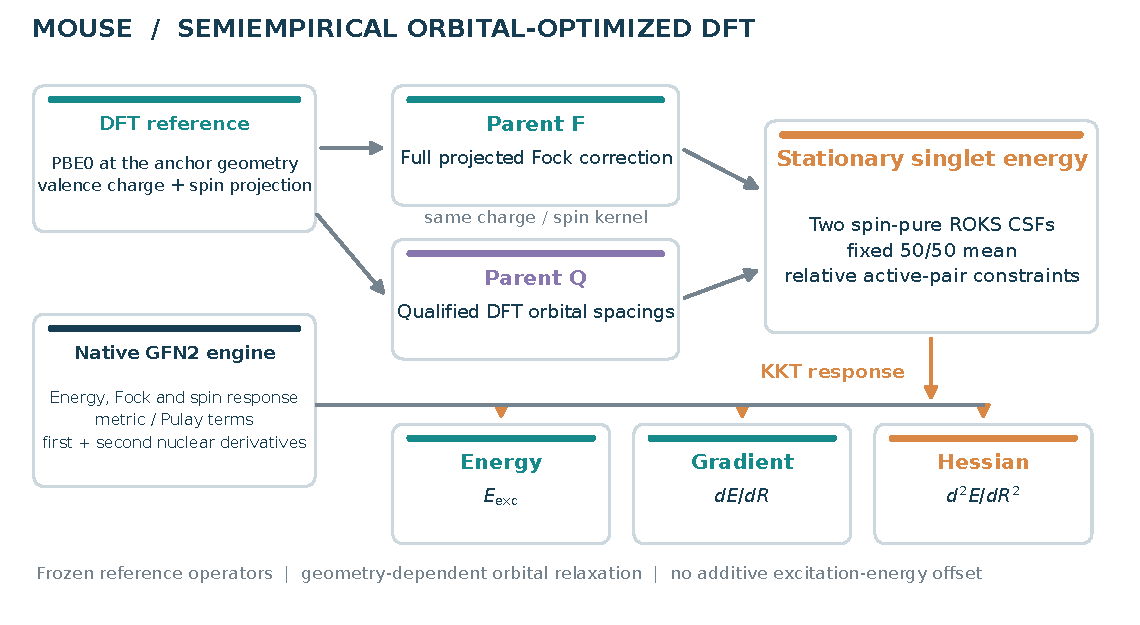
\includegraphics[width=0.82\linewidth]{figures/method_workflow.pdf}
\end{center}
\noindent\emph{TOC text:} A prepared DFT-informed semiempirical surface
combines spin-pure orbital optimization, coherent state interaction and
analytic nuclear response for repeated excited-state calculations.

\setlength{\bibsep}{2pt}
\begin{thebibliography}{35}
\providecommand{\natexlab}[1]{#1}
\providecommand{\url}[1]{\texttt{#1}}
\expandafter\ifx\csname urlstyle\endcsname\relax
  \providecommand{\doi}[1]{doi: #1}\else
  \providecommand{\doi}{doi: \begingroup \urlstyle{rm}\Url}\fi

\bibitem[Chung et~al.(2015)Chung, Sameera, Ramozzi, Page, Hatanaka, Petrova,
  Harris, Li, Ke, Liu, Li, Ding, and Morokuma]{oniom2015}
Lung~Wa Chung, W.~M.~C. Sameera, Romain Ramozzi, Alister~J. Page, Miho
  Hatanaka, Galina~P. Petrova, Travis~V. Harris, Xin Li, Zhuofeng Ke, Fengyi
  Liu, Hai-Bei Li, Lina Ding, and Keiji Morokuma.
\newblock The {ONIOM} method and its applications.
\newblock \emph{Chemical Reviews}, 115\penalty0 (12):\penalty0 5678--5796,
  2015.
\newblock \doi{10.1021/cr5004419}.

\bibitem[Grimme(2013)]{tda}
Stefan Grimme.
\newblock {A simplified Tamm-Dancoff density functional approach for the
  electronic excitation spectra of very large molecules}.
\newblock \emph{The Journal of Chemical Physics}, 138:\penalty0 244104, 2013.
\newblock \doi{10.1063/1.4811331}.

\bibitem[Bannwarth and Grimme(2014)]{stdft2014}
Christoph Bannwarth and Stefan Grimme.
\newblock {A simplified time-dependent density functional theory approach for
  electronic ultraviolet and circular dichroism spectra of very large
  molecules}.
\newblock \emph{Computational and Theoretical Chemistry}, 1040-1041:\penalty0
  45--53, 2014.
\newblock \doi{10.1016/j.comptc.2014.02.023}.

\bibitem[Grimme and Bannwarth(2016)]{stdaxtb2016}
Stefan Grimme and Christoph Bannwarth.
\newblock {Ultra-fast computation of electronic spectra for large systems by
  tight-binding based simplified Tamm-Dancoff approximation (sTDA-xTB)}.
\newblock \emph{The Journal of Chemical Physics}, 145:\penalty0 054103, 2016.
\newblock \doi{10.1063/1.4959605}.

\bibitem[Beaujean et~al.(2026)Beaujean, Liger, Satisha, Maraldi, Bannwarth, and
  de~Wergifosse]{std22026}
Pierre Beaujean, Axel Liger, Arya Satisha, Marilù~G. Maraldi, Christoph
  Bannwarth, and Marc de~Wergifosse.
\newblock {The std2 package: A computationally efficient program to calculate
  molecular response properties and excited states using simplified quantum
  chemistry methods}.
\newblock \emph{The Journal of Chemical Physics}, 165:\penalty0 152501, 2026.
\newblock \doi{10.1063/5.0349975}.

\bibitem[Hourahine et~al.(2025)Hourahine, Berdakin, Bich, Bonaf{\'e}, Camacho,
  Cui, Deshaye, Díaz~Mir{\'o}n, Ehlert, Elstner, Frauenheim, Goldman,
  González~Le{\'o}n, van~der Heide, Irle, Kowalczyk, Kubař, Lee,
  Lien-Medrano, Maryewski, Melson, Min, Niehaus, Niklasson, Pecchia, Reuter,
  Sánchez, Scheurer, Sentef, Stishenko, Vuong, and Aradi]{dftb2025}
B.~Hourahine, M.~Berdakin, J.~A. Bich, F.~P. Bonaf{\'e}, C.~Camacho, Q.~Cui,
  M.~Y. Deshaye, G.~Díaz~Mir{\'o}n, S.~Ehlert, M.~Elstner, T.~Frauenheim,
  N.~Goldman, R.~A. González~Le{\'o}n, T.~van~der Heide, S.~Irle,
  T.~Kowalczyk, T.~Kubař, I.~S. Lee, C.~R. Lien-Medrano, A.~Maryewski,
  T.~Melson, S.~K. Min, T.~Niehaus, A.~M.~N. Niklasson, A.~Pecchia, K.~Reuter,
  C.~G. Sánchez, C.~Scheurer, M.~A. Sentef, P.~V. Stishenko, V.~Q. Vuong, and
  B.~Aradi.
\newblock {Recent Developments in DFTB+, a Software Package for Efficient
  Atomistic Quantum Mechanical Simulations}.
\newblock \emph{The Journal of Physical Chemistry A}, 129:\penalty0 5373--5390,
  2025.
\newblock \doi{10.1021/acs.jpca.5c01146}.

\bibitem[Kowalczyk et~al.(2016)Kowalczyk, Le, and Irle]{deltadftb2016}
Tim Kowalczyk, Khoa Le, and Stephan Irle.
\newblock {Self-Consistent Optimization of Excited States within
  Density-Functional Tight-Binding}.
\newblock \emph{Journal of Chemical Theory and Computation}, 12:\penalty0
  313--323, 2016.
\newblock \doi{10.1021/acs.jctc.5b00734}.

\bibitem[Havenridge et~al.(2023)Havenridge, R{\"u}ger, and Aikens]{tbgrad2023}
Shana Havenridge, Robert R{\"u}ger, and Christine~M. Aikens.
\newblock {Analytical excited state gradients for time-dependent density
  functional theory plus tight binding (TDDFT + TB)}.
\newblock \emph{The Journal of Chemical Physics}, 158:\penalty0 224103, 2023.
\newblock \doi{10.1063/5.0142240}.

\bibitem[Wang et~al.(2024)Wang, Havenridge, and Aikens]{aas2024}
Yuchen Wang, Shana Havenridge, and Christine~M. Aikens.
\newblock {Implementation of energy and gradient for the TDDFT-approximate
  auxiliary function (aas) method}.
\newblock \emph{The Journal of Chemical Physics}, 161:\penalty0 024101, 2024.
\newblock \doi{10.1063/5.0213587}.

\bibitem[Tuna et~al.(2016)Tuna, Lu, Koslowski, and Thiel]{omxexc2016}
Deniz Tuna, You Lu, Axel Koslowski, and Walter Thiel.
\newblock {Semiempirical Quantum-Chemical Orthogonalization-Corrected Methods:
  Benchmarks of Electronically Excited States}.
\newblock \emph{Journal of Chemical Theory and Computation}, 12:\penalty0
  4400--4422, 2016.
\newblock \doi{10.1021/acs.jctc.6b00403}.

\bibitem[Dral et~al.(2019)Dral, Wu, and Thiel]{odmx2019}
Pavlo~O. Dral, Xin Wu, and Walter Thiel.
\newblock {Semiempirical Quantum-Chemical Methods with Orthogonalization and
  Dispersion Corrections}.
\newblock \emph{Journal of Chemical Theory and Computation}, 15:\penalty0
  1743--1760, 2019.
\newblock \doi{10.1021/acs.jctc.8b01265}.

\bibitem[Gilbert et~al.(2008)Gilbert, Besley, and Gill]{mom2008}
Andrew T.~B. Gilbert, Nicholas~A. Besley, and Peter M.~W. Gill.
\newblock Self-consistent field calculations of excited states using the
  maximum overlap method ({MOM}).
\newblock \emph{The Journal of Physical Chemistry A}, 112\penalty0
  (50):\penalty0 13164--13171, 2008.
\newblock \doi{10.1021/jp801738f}.

\bibitem[Hait and Head-Gordon(2021)]{hait2021}
Diptarka Hait and Martin Head-Gordon.
\newblock Orbital optimized density functional theory for electronic excited
  states.
\newblock \emph{The Journal of Physical Chemistry Letters}, 12\penalty0
  (19):\penalty0 4517--4529, 2021.
\newblock \doi{10.1021/acs.jpclett.1c00744}.

\bibitem[Levi et~al.(2020{\natexlab{a}})Levi, Ivanov, and
  J{\'o}nsson]{levifaraday}
Gianluca Levi, Aleksei~V. Ivanov, and Hannes J{\'o}nsson.
\newblock {Variational calculations of excited states via direct optimization
  of the orbitals in DFT}.
\newblock \emph{Faraday Discussions}, 224:\penalty0 448--466,
  2020{\natexlab{a}}.
\newblock \doi{10.1039/D0FD00064G}.

\bibitem[Levi et~al.(2020{\natexlab{b}})Levi, Ivanov, and
  J{\'o}nsson]{levi2020}
Gianluca Levi, Aleksei~V. Ivanov, and Hannes J{\'o}nsson.
\newblock {Variational Density Functional Calculations of Excited States via
  Direct Optimization}.
\newblock \emph{Journal of Chemical Theory and Computation}, 16:\penalty0
  6968--6982, 2020{\natexlab{b}}.
\newblock \doi{10.1021/acs.jctc.0c00597}.

\bibitem[Ivanov et~al.(2021)Ivanov, Levi, J{\'o}nsson, and
  J{\'o}nsson]{ivanov2021}
Aleksei~V. Ivanov, Gianluca Levi, Elvar~{\"O}. J{\'o}nsson, and Hannes
  J{\'o}nsson.
\newblock {Method for Calculating Excited Electronic States Using Density
  Functionals and Direct Orbital Optimization with Real Space Grid or
  Plane-Wave Basis Set}.
\newblock \emph{Journal of Chemical Theory and Computation}, 17:\penalty0
  5034--5049, 2021.
\newblock \doi{10.1021/acs.jctc.1c00157}.

\bibitem[Schmerwitz et~al.(2023)Schmerwitz, Levi, and J{\'o}nsson]{gmf2023}
Yorick L.~A. Schmerwitz, Gianluca Levi, and Hannes J{\'o}nsson.
\newblock {Calculations of Excited Electronic States by Converging on Saddle
  Points Using Generalized Mode Following}.
\newblock \emph{Journal of Chemical Theory and Computation}, 19:\penalty0
  3634--3651, 2023.
\newblock \doi{10.1021/acs.jctc.3c00178}.

\bibitem[Bannwarth et~al.(2019)Bannwarth, Ehlert, and Grimme]{gfn2}
Christoph Bannwarth, Sebastian Ehlert, and Stefan Grimme.
\newblock {{GFN2-xTB}: An Accurate and Broadly Parametrized Self-Consistent
  Tight-Binding Quantum Chemical Method with Multipole Electrostatics and
  Density-Dependent Dispersion Contributions}.
\newblock \emph{Journal of Chemical Theory and Computation}, 15:\penalty0
  1652--1671, 2019.
\newblock \doi{10.1021/acs.jctc.8b01176}.

\bibitem[Frank et~al.(1998)Frank, Hutter, Marx, and Parrinello]{roks1998}
Irmgard Frank, J{\"u}rg Hutter, Dominik Marx, and Michele Parrinello.
\newblock {Molecular dynamics in low-spin excited states}.
\newblock \emph{The Journal of Chemical Physics}, 108:\penalty0 4060--4069,
  1998.
\newblock \doi{10.1063/1.475804}.

\bibitem[Yanai et~al.(2004)Yanai, Tew, and Handy]{camb3lyp2004}
Takeshi Yanai, David~P. Tew, and Nicholas~C. Handy.
\newblock A new hybrid exchange--correlation functional using the
  coulomb-attenuating method ({CAM-B3LYP}).
\newblock \emph{Chemical Physics Letters}, 393:\penalty0 51--57, 2004.
\newblock \doi{10.1016/j.cplett.2004.06.011}.

\bibitem[V{\'e}ril et~al.(2021)V{\'e}ril, Scemama, Caffarel, Lipparini,
  Boggio‐Pasqua, Jacquemin, and Loos]{quest}
Micka{\"e}l V{\'e}ril, Anthony Scemama, Michel Caffarel, Filippo Lipparini,
  Martial Boggio‐Pasqua, Denis Jacquemin, and Pierre‐Fran{\c c}ois Loos.
\newblock {QUESTDB: A database of highly accurate excitation energies for the
  electronic structure community}.
\newblock \emph{WIREs Computational Molecular Science}, 11:\penalty0 e1517,
  2021.
\newblock \doi{10.1002/wcms.1517}.

\bibitem[Loos et~al.(2025)Loos, Boggio-Pasqua, Blondel, Lipparini, and
  Jacquemin]{quest2025}
Pierre-Fran{\c c}ois Loos, Martial Boggio-Pasqua, Aymeric Blondel, Filippo
  Lipparini, and Denis Jacquemin.
\newblock {{QUEST} Database of Highly-Accurate Excitation Energies}.
\newblock \emph{Journal of Chemical Theory and Computation}, 21:\penalty0
  8010--8033, 2025.
\newblock \doi{10.1021/acs.jctc.5c00975}.

\bibitem[Aryasetiawan et~al.(2004)Aryasetiawan, Imada, Georges, Kotliar,
  Biermann, and Lichtenstein]{crpa2004}
F.~Aryasetiawan, M.~Imada, A.~Georges, G.~Kotliar, S.~Biermann, and A.~I.
  Lichtenstein.
\newblock Frequency-dependent local interactions and low-energy effective
  models from electronic structure calculations.
\newblock \emph{Physical Review B}, 70:\penalty0 195104, 2004.
\newblock \doi{10.1103/PhysRevB.70.195104}.

\bibitem[R{\"u}ger et~al.(2016)R{\"u}ger, Niehaus, van Lenthe, Heine, and
  Visscher]{tddftbvib2016}
Robert R{\"u}ger, Thomas Niehaus, Erik van Lenthe, Thomas Heine, and Lucas
  Visscher.
\newblock {Vibrationally resolved UV/Vis spectroscopy with time-dependent
  density functional based tight binding}.
\newblock \emph{The Journal of Chemical Physics}, 145:\penalty0 184102, 2016.
\newblock \doi{10.1063/1.4966918}.

\bibitem[Budzák et~al.(2017)Budzák, Scalmani, and Jacquemin]{geometries2017}
Šimon Budzák, Giovanni Scalmani, and Denis Jacquemin.
\newblock {Accurate Excited-State Geometries: A CASPT2 and Coupled-Cluster
  Reference Database for Small Molecules}.
\newblock \emph{Journal of Chemical Theory and Computation}, 13:\penalty0
  6237--6252, 2017.
\newblock \doi{10.1021/acs.jctc.7b00921}.

\bibitem[Job et~al.(1969)Job, Sethuraman, and Innes]{formaldehydespectrum1969}
V.~A. Job, V.~Sethuraman, and K.~K. Innes.
\newblock The 3500 {\aa} transition of formaldehyde-h2, d2, and hd: Vibrational
  and rotational analyses.
\newblock \emph{Journal of Molecular Spectroscopy}, 30:\penalty0 365--426,
  1969.
\newblock \doi{10.1016/0022-2852(69)90274-4}.

\bibitem[Hubbard et~al.(1981)Hubbard, Bocian, and
  Birge]{acetaldehydespectrum1981}
Lynn~M. Hubbard, David~F. Bocian, and Robert~R. Birge.
\newblock The nature of the {$^1n\pi^*\leftarrow S_0$} transition. 4. the first
  excited singlet state of acetaldehyde.
\newblock \emph{Journal of the American Chemical Society}, 103:\penalty0
  3313--3320, 1981.
\newblock \doi{10.1021/ja00402a016}.

\bibitem[Miyake et~al.(2009)Miyake, Aryasetiawan, and Imada]{miyake2009}
Takashi Miyake, Ferdi Aryasetiawan, and Masatoshi Imada.
\newblock Ab initio procedure for constructing effective models of correlated
  materials with entangled band structure.
\newblock \emph{Physical Review B}, 80:\penalty0 155134, 2009.
\newblock \doi{10.1103/PhysRevB.80.155134}.

\bibitem[Verzijl and F{\"o}rster(2026)]{verzijl2026}
Erik Verzijl and Arno F{\"o}rster.
\newblock Static effective hamiltonians for molecular systems through
  {RPA}-based downfolding.
\newblock \emph{Journal of Chemical Theory and Computation}, 22\penalty0
  (18):\penalty0 9468--9482, 2026.
\newblock \doi{10.1021/acs.jctc.6c01128}.

\bibitem[Schmerwitz et~al.(2026)Schmerwitz, Selenius, and Levi]{freeze2026}
Yorick L.~A. Schmerwitz, Elli Selenius, and Gianluca Levi.
\newblock {Freeze-and-Release Direct Optimization Method for Variational
  Calculations of Excited Electronic States}.
\newblock \emph{Journal of Chemical Theory and Computation}, 22:\penalty0
  3571--3584, 2026.
\newblock \doi{10.1021/acs.jctc.5c01974}.

\bibitem[Bondarev and Knyukshto(1994)]{Bondarev1994}
S.~L. Bondarev and V.~N. Knyukshto.
\newblock Fluorescence from the {S1} state of all-trans-beta-carotene.
\newblock \emph{Chemical Physics Letters}, 225:\penalty0 346--350, 1994.
\newblock \doi{10.1016/0009-2614(94)87092-6}.

\bibitem[Clementson and Wojtasiewicz(2019)]{Clementson2019}
Lesley~A. Clementson and Bozena Wojtasiewicz.
\newblock Dataset on the absorption characteristics of extracted phytoplankton
  pigments.
\newblock \emph{Data in Brief}, 24:\penalty0 103875, 2019.
\newblock \doi{10.1016/j.dib.2019.103875}.

\bibitem[Marian et~al.(2019)Marian, Heil, and Kleinschmidt]{marian2019mrci}
Christel~M. Marian, Adrian Heil, and Martin Kleinschmidt.
\newblock The dft/mrci method.
\newblock \emph{WIREs Computational Molecular Science}, 9:\penalty0 e1394,
  2019.
\newblock \doi{10.1002/wcms.1394}.

\bibitem[Tselyaev(2013)]{tselyaev2013}
V.~I. Tselyaev.
\newblock Subtraction method and stability condition in extended random-phase
  approximation theories.
\newblock \emph{Physical Review C}, 88:\penalty0 054301, 2013.
\newblock \doi{10.1103/PhysRevC.88.054301}.

\bibitem[Gambacurta et~al.(2015)Gambacurta, Grasso, and Engel]{gambacurta2015}
D.~Gambacurta, M.~Grasso, and J.~Engel.
\newblock Subtraction method in the second random-phase approximation: First
  applications with a skyrme energy functional.
\newblock \emph{Physical Review C}, 92:\penalty0 034303, 2015.
\newblock \doi{10.1103/PhysRevC.92.034303}.

\end{thebibliography}

\end{document}
